\documentclass[t]{beamer}
\mode<presentation>

\usepackage{etex}

\usetheme{Madrid}
% other themes: Warsaw, AnnArbor, Antibes, Bergen, Berkeley, Berlin, Boadilla, boxes, CambridgeUS, Copenhagen, Darmstadt, default, Dresden, Frankfurt, Goettingen,
% Hannover, Ilmenau, JuanLesPins, Luebeck, Madrid, Maloe, Marburg, Montpellier, PaloAlto, Pittsburg, Rochester, Singapore, Szeged, classic

\setbeamertemplate{navigation symbols}{\insertslidenavigationsymbol}

\usecolortheme{dolphin}
%\usecolortheme{seagull}
% color themes: albatross, beaver, beetle, crane, default, dolphin, dov, fly, lily, orchid, rose, seagull, seahorse, sidebartab, structure, whale, wolverine

%\usefonttheme{serif}
% font themes: default, professionalfonts, serif, structurebold, structureitalicserif, structuresmallcapsserif

% pdf is displayed in full screen mode automatically
%\hypersetup{pdfpagemode=FullScreen}

%\AtBeginSection[]
%{
%  \begin{frame}<beamer>
%    \frametitle{Outline}
%    \tableofcontents[currentsection,currentsubsection]
%  \end{frame}
%}

% define your own colours:
\definecolor{Red}{rgb}{1,0,0}
\definecolor{Blue}{rgb}{0,0,1}
\definecolor{Green}{rgb}{0,1,0}
\definecolor{magenta}{rgb}{1,0,.6}
\definecolor{lightblue}{rgb}{0,.8,1}
\definecolor{lightpurple}{rgb}{.6,.4,1}
\definecolor{gold}{rgb}{.6,.5,0}
\definecolor{orange}{rgb}{1,0.4,0}
\definecolor{hotpink}{rgb}{1,0,0.5}
\definecolor{newcolor2}{rgb}{.5,.3,.5}
\definecolor{newcolor}{rgb}{0,.3,1}
\definecolor{newcolor3}{rgb}{1,0,.35}
\definecolor{darkgreen1}{rgb}{0, .35, 0}
\definecolor{darkgreen}{rgb}{0, .6, 0}
\definecolor{darkred}{rgb}{.75,0,0}

\xdefinecolor{olive}{cmyk}{0.64,0,0.95,0.4}
\xdefinecolor{purpleish}{cmyk}{0.75,0.75,0,0}

%\usepackage{beamerinnerthemerounded}
% inner themes include circles, default, inmargin, rectangles, rounded

%\usepackage{beamerouterthemesmoothbars}
% outer themes include default, infolines, miniframes, shadow, sidebar, smoothbars, smoothtree, split, tree

\useoutertheme[subsection=false]{smoothbars}

% to have the same footer on all slides
\setbeamertemplate{footline}[text line]{

\includegraphics[height=15pt]{sulogolong.eps}\hfill 
\raisebox{5pt}{Math 207:  Introduction to Statistics}\hfill 
\raisebox{5pt}{Chapter 9: More About Correlation}\hfill
\raisebox{5pt}{\insertframenumber/\pageref{lastpage}}}
%\setbeamertemplate{footline}[text line]{} % or empty footer

% include packages
\usepackage{subfigure}
\usepackage{multicol}
\usepackage{amsmath}
\usepackage{epsfig}
\usepackage{graphicx}
\usepackage[all,knot]{xy}
\xyoption{arc}
\usepackage{url}
\usepackage{multimedia}
\usepackage{hyperref}
\usepackage{setspace}

\title{Math 207:  Statistics}
\subtitle{Chapter 9:  More About Correlation}
\author{Ralph Wojtowicz}
\institute{Mathematics Department\\ Shenandoah University}
%\date{\scriptsize 16 September 2011}

\usepackage{pstricks,pst-grad,pst-func,pst-text,pst-node,multido,pst-plot,calc,pst-3dplot}

\newcommand{\BRACE}{
\begin{pspicture}(-3,-2.1)(3,1.1)
\psset{yunit=3,linewidth=0.02}
\psline(-3.5,0)(3.5,0)  
  \psline(-3,0)(-3,-0.04) \rput[t](-3,-0.07){\scriptsize -3\hphantom{-}}
  \psline(-2,0)(-2,-0.04) \rput[t](-2,-0.07){\scriptsize -2\hphantom{-}}
  \psline(-1,0)(-1,-0.04) \rput[t](-1,-0.07){\scriptsize -1\hphantom{-}}
  \psline(0,0)(0,-0.04)   \rput[t](0,-0.07){\scriptsize 0}
  \psline(1,0)(1,-0.04)   \rput[t](1,-0.07){\scriptsize 1}
  \psline(2,0)(2,-0.04)   \rput[t](2,-0.07){\scriptsize 2}
  \psline(3,0)(3,-0.04)   \rput[t](3,-0.07){\scriptsize 3}
  \rput[l](3.6,0){\scriptsize $x$}
\psline(0,0)(0,0.5)
  \psline(-0.12,0.5)(0,0.5)    \rput[r](-0.21,0.5){\scriptsize $0.5$}
  \psline(-0.12,0.25)(0,0.25)  \rput[r](-0.21,0.25){\scriptsize $0.25$}
\psGauss[linecolor=blue,linewidth=0.02,sigma=1,mue=0]{-3}{3}
\pnode(-1,-0.15){A}\pnode(1,-0.15){B}
\psbrace[braceWidth=0.02,braceWidthInner=5pt,braceWidthOuter=5pt](A)(B){\rput{90}(0.25,-0.05){\scriptsize 68\%}}
%
\pnode(-2,-0.15){C}\pnode(2,-0.15){D}
\psbrace[braceWidth=0.02,braceWidthInner=25pt,braceWidthOuter=5pt](C)(D){\rput{90}(0.25,-0.05){\scriptsize 95\%}}
%
\pnode(-3,-0.15){E}\pnode(3,-0.15){F}
\psbrace[braceWidth=0.02,braceWidthInner=45pt,braceWidthOuter=5pt](E)(F){\rput{90}(0.25,-0.1){\scriptsize 99.7\%}}
\end{pspicture}}

\definecolor{Red}{rgb}{1,0,0}
\definecolor{Blue}{rgb}{0,0,1}
\definecolor{Green}{rgb}{0,1,0}
\definecolor{magenta}{rgb}{1,0,.6}
\definecolor{lightblue}{rgb}{0,.8,1}
\definecolor{lightpurple}{rgb}{.6,.4,1}
\definecolor{gold}{rgb}{.6,.5,0}
\definecolor{orange}{rgb}{1,0.4,0}
\definecolor{hotpink}{rgb}{1,0,0.5}
\definecolor{newcolor2}{rgb}{.5,.3,.5}
\definecolor{newcolor}{rgb}{0,.3,1}
\definecolor{newcolor3}{rgb}{1,0,.35}
\definecolor{darkgreen1}{rgb}{0, .35, 0}
\definecolor{darkgreen}{rgb}{0, .4, 0}
\definecolor{medgreen}{rgb}{0, .6, 0}
\definecolor{darkred}{rgb}{.75,0,0}
\definecolor{gold}{rgb}{0.85, 0.65, 0.13}
\definecolor{dgreen}{rgb}{0.0, 0.39, 0.0}
\definecolor{tbc}{rgb}{0.0, 0.6, 0.6}
\definecolor{ads}{rgb}{0.6, 0.0, 0.6}
\definecolor{silver}{rgb}{0.6, 0.6, 0.6}
\definecolor{platinum}{rgb}{0.5, 0.5, 0.4}
\definecolor{copper}{rgb}{0.722, 0.4824, 0.4196}

\xdefinecolor{olive}{cmyk}{0.64,0,0.95,0.4}
\xdefinecolor{purpleish}{cmyk}{0.75,0.75,0,0}


\begin{document}

%\frame[plain]{
%	\titlepage
%}


\begin{frame}[plain]
\definecolor{myblue}{rgb}{0,0,0.6}
\definecolor{grayA}{rgb}{0.95,0.95,0.95}
\definecolor{grayB}{rgb}{0.98,0.98,0.98}
\begin{center}

%\begin{pspicture}(0,0)(7,4.8)
\begin{pspicture}(-6,-7)(6,2)
\rput(0,-1.85){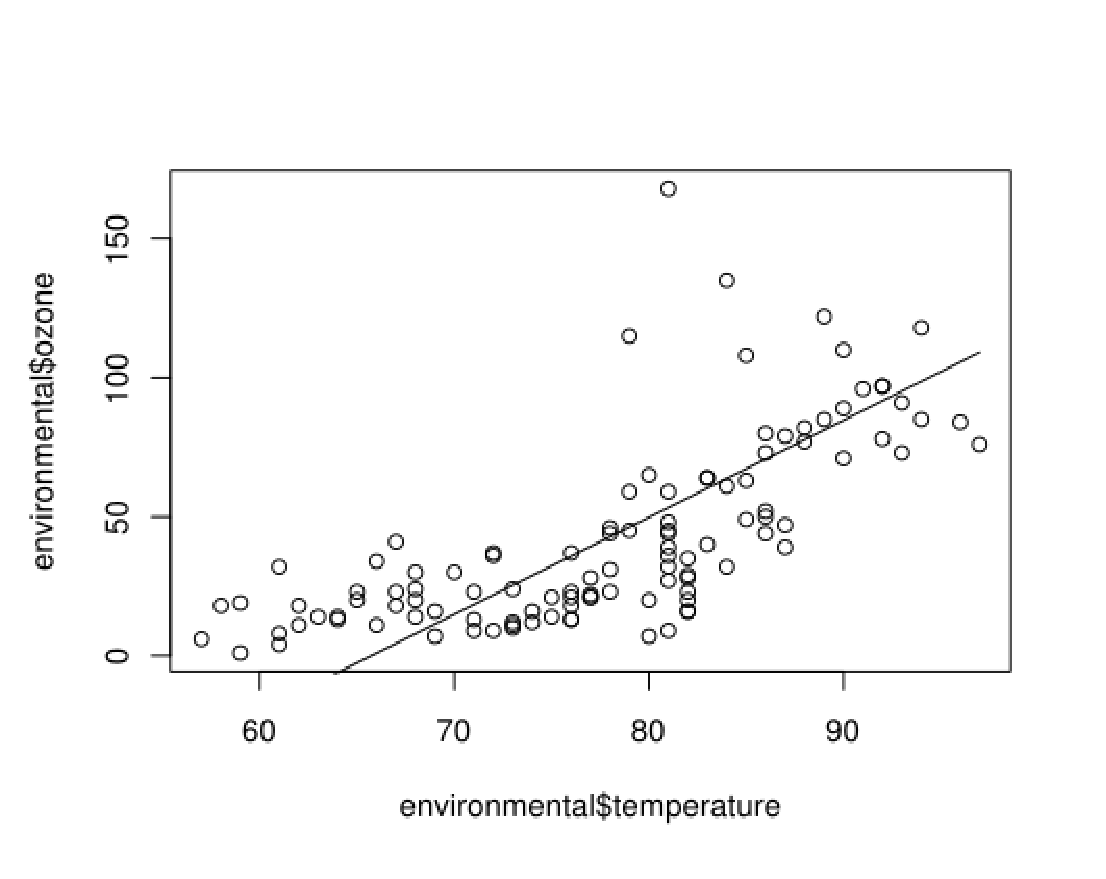
\includegraphics[height=4.2cm,bb=-0 -0 515 350,clip]{ozoneLine.eps}}
\psframe[linewidth=0.02,linecolor=gray](-6.2,-7)(6.2,2.2)
\psframe[linewidth=0.02,linecolor=gray](-6.15,-6.95)(6.15,2.15)
\rput(0,1.4){\color{myblue}\large Math 207:  Statistics}
\rput(0,0.6){\color{myblue}Chapter 9:  More about Correlation}
%\psframebox(0,0)(4,4)
%\rput(0,-4.4){\scriptsize Dr.~Ralph Wojtowicz}
%\rput(0,-4.9){\scriptsize CME Department}
\rput(0,-5.6){
\includegraphics[height=2cm]{sulogolong.eps}}
%
%\rput(0,-6.5){\scriptsize 14 September 2011}
\end{pspicture}
\end{center}

\end{frame}

%\section[Outline]{}

\addtocounter{page}{-1}
\addtocounter{framenumber}{-1}

{\footnotesize
\frame{\tableofcontents}
}

\section{Features}
\subsection{Features}
\begin{frame}[t]\frametitle{Features of the Correlation Coefficient}
{\small
\begin{itemize}
\item Given lists $x_1$, $\dots$, $x_n$ and $y_1$, $\dots$, $y_n$, the correlation
  coefficient $r$:
  \begin{itemize} 
     \item \footnotesize  is a measure of linear association between the lists,
     \item \footnotesize  is a measure of the clustering of the $(x_i, y_i)$ points around a line,
     \item \footnotesize  is a number between $-1$ and $1$ and
     \item \footnotesize  is defined by:\vspace{-10pt}
   \end{itemize}
\end{itemize}
\begin{align*}
r &=\frac{1}{n}\,\sum_{i=1}^n\,\left(\frac{x_i - \mbox{mean}_x}{\mbox{SD}_x}\right)\,
  \left(\frac{y_i - \mbox{mean}_y}{\mbox{SD}_y}\right)\\
  &= \mbox{average of the $x$ and $y$ values measured in standard units}\vspace{-20pt}
\end{align*}\vspace{-15pt}
\begin{itemize}
\item $r$ is a number with no units (if $x$ is in feet, for example, then $\mbox{mean}_x$ and
   $\mbox{SD}_x$ are also in feet so the units cancel).
\item Transformations that don't change the correlation:
   \begin{itemize}
   \item \footnotesize Reversing the variables: $\mbox{cor}(x,\,y) = \mbox{cor}(y,\,x)$
   \item \footnotesize  Shifting one (or both) variables: $\mbox{cor}(x + A,\,y) = \mbox{cor}(y,\,x)$
   \item \footnotesize  Scaling one (or both) variables: $\mbox{cor}(B\,x,\,y) = \mbox{cor}(y,\,x)$
   \end{itemize}
\end{itemize}

}
\end{frame}

\begin{frame}
\frametitle{Transforming Variables}
\small
{\ }\vspace{-10pt}

\begin{center}
\begin{pspicture}(-3,0.4)(5,3.5)
\psset{xunit=0.02, yunit=0.11}
\psdots*[fillcolor=blue,linecolor=blue](110,21)(110,21)(93,22.8)(110,21.4)(175,18.7)(105,18.1)(245,14.3)(62,24.4)(95,22.8)(123,19.2)(123,17.8)(180,16.4)(180,17.3)(180,15.2)(205,10.4)(215,10.4)(230,14.7)(66,32.4)(52,30.4)(65,33.9)(97,21.5)(150,15.5)(150,15.2)(245,13.3)(175,19.2)(66,27.3)(91,26)(113,30.4)(264,15.8)(175,19.7)(335,15)(109,21.4)
\psaxes[Dx=50,Dy=5](0,0)(350,0)(0,35)
\rput(200,-8){Horsepower}
\rput{90}(-50,17.5){Miles per Gallon}
\end{pspicture}
\end{center}

\scriptsize

\begin{itemize}
\item Compare:\\
\texttt{> $\mbox{cor}(\mbox{mtcars}\$\mbox{hp},\; \mbox{mtcars}\$\mbox{mpg})$}\\
\texttt{[1] -0.7761684}\\[3pt]
\texttt{> $\mbox{cor}(\mbox{mtcars}\$\mbox{hp},\; \mbox{mtcars}\$\mbox{mpg} - 30)$}\\
\texttt{[1] -0.7761684}\\[3pt]
\texttt{> $\mbox{cor}(\mbox{mtcars}\$\mbox{hp},\; 0.425 * \mbox{mtcars}\$\mbox{mpg})$}
    \ \ \ \# Convert to km / liter.\\
\texttt{[1] -0.7761684}\\[3pt]
\texttt{> $\mbox{cor}(\mbox{mtcars}\$\mbox{mpg},\; \mbox{mtcars}\$\mbox{hp})$}\\
\texttt{[1] -0.7761684}\\
\end{itemize}
\end{frame}

\section{Nonlinearity}
\subsection{Nonlinearity}
\begin{frame}
\frametitle{Nonlinearity}
\footnotesize

\begin{itemize}
\item Correlation measures {\color{blue}linear association} between variables.
\item It does not caputure  nonlinear association between  variables.
\item Example:  The  variables shown below have a strong quadratic association but 
their correlation is $-0.017$.
\end{itemize}

\begin{center}
\begin{pspicture}(-2,0)(2,4)
\psdots*[fillcolor=blue,linecolor=blue](-2,3.99426031420378)(-1.8,3.29826862826557)(-1.6,2.65385611936148)(-1.4,1.91366298768045)(-1.2,1.50873490635927)(-1,0.86518773484837)(-0.8,0.727591083136367)(-0.6,0.382252947267038)(-0.4,0.239127249749482)(-0.2,0.213173719370425)(0,0.0180257620941494)(0.2,0.0752876993477757)(0.4,0.0929653439222215)(0.6,0.254113025833174)(0.8,0.509623629422163)(1,1.14302160708342)(1.2,1.23063632968958)(1.4,1.91899723716125)(1.6,2.64954195956695)(1.8,3.28280464741336)(2,3.9189188731987)
\psaxes(0,0)(-2,0)(2,4)
\end{pspicture}
\end{center}

\end{frame}

\section{Association}
\subsection{Association}
\begin{frame}[t]\frametitle{Association is Not Causation!}
{\footnotesize

\begin{itemize}
\item Correlation measures association.  But {\color{blue}association is not the same as causation}.
\item Two variables may have a strong positive or negative correlation without having one
   causing the other to change.  The change may be due to some other, confounding factor.
\item Example:  gold and government bond prices tend to move in opposite directions.\\
    There is a strong negative correlation.
    Other economic factors  can lead investors  to move funds
      out of  bonds into something that will hold a stable value.\vspace{5pt}
\end{itemize}

\begin{center}
\scalebox{0.65}{\begin{pspicture}(-0.6, -1.1 )( 14.7 , 4.7 )
\psset{linewidth=0.02}
\rput(7,4.8){\large Daily gold prices  and 10-year real yield rates}
\psset{xunit= 0.00350156966916204 }
\psset{yunit= 0.0025 }
\psline(0,0)( 4141 , 0)
\rput[r]{45}( , -120 ){\small  }
\psline[linestyle=dotted]( ,  -96 )( , 2000 )
\rput[r]{45}( 342 , -120 ){\scriptsize  2003-12-10 }
\psline[linestyle=dotted]( 342 ,  -96 )( 342 , 2000 )
\rput[r]{45}( 687 , -120 ){\scriptsize  2004-11-19 }
\psline[linestyle=dotted]( 687 ,  -96 )( 687 , 2000 )
\rput[r]{45}( 1030 , -120 ){\scriptsize  2005-10-28 }
\psline[linestyle=dotted]( 1030 ,  -96 )( 1030 , 2000 )
\rput[r]{45}( 1377 , -120 ){\scriptsize  2006-10-10 }
\psline[linestyle=dotted]( 1377 ,  -96 )( 1377 , 2000 )
\rput[r]{45}( 1719 , -120 ){\scriptsize  2007-09-17 }
\psline[linestyle=dotted]( 1719 ,  -96 )( 1719 , 2000 )
\rput[r]{45}( 2063 , -120 ){\scriptsize  2008-08-26 }
\psline[linestyle=dotted]( 2063 ,  -96 )( 2063 , 2000 )
\rput[r]{45}( 2408 , -120 ){\scriptsize  2009-08-06 }
\psline[linestyle=dotted]( 2408 ,  -96 )( 2408 , 2000 )
\rput[r]{45}( 2752 , -120 ){\scriptsize  2010-07-16 }
\psline[linestyle=dotted]( 2752 ,  -96 )( 2752 , 2000 )
\rput[r]{45}( 3095 , -120 ){\scriptsize  2011-06-24 }
\psline[linestyle=dotted]( 3095 ,  -96 )( 3095 , 2000 )
\rput[r]{45}( 3441 , -120 ){\scriptsize  2012-06-04 }
\psline[linestyle=dotted]( 3441 ,  -96 )( 3441 , 2000 )
\rput[r]{45}( 3786 , -120 ){\scriptsize  2013-05-15 }
\psline[linestyle=dotted]( 3786 ,  -96 )( 3786 , 2000 )
\rput[r]{45}( 4131 , -120 ){\scriptsize  2014-04-25 }
\psline[linestyle=dotted]( 4131 ,  -96 )( 4131 , 2000 )

\psline[linecolor= gold ]( 0 , 343.8 )( 1 , 344.5 )( 4 , 351.75 )( 5 , 349 )( 6 , 349.75 )( 7 , 352.4 )( 8 , 353 )( 11 , 352.55 )( 12 , 353.1 )( 13 , 351 )( 14 , 352.3 )( 15 , 357 )( 19 , 353.8 )( 20 , 358.5 )( 21 , 364.7 )( 22 , 366 )( 25 , 368.5 )( 26 , 368.4 )( 27 , 369.9 )( 28 , 367.6 )( 29 , 367.5 )( 32 , 369.5 )( 33 , 376.55 )( 34 , 382.1 )( 35 , 375.8 )( 36 , 373.25 )( 39 , 370.5 )( 40 , 364 )( 41 , 356.3 )( 42 , 352.8 )( 43 , 354.25 )( 47 , 344.1 )( 48 , 346 )( 49 , 351.55 )( 50 , 352.3 )( 53 , 355.2 )( 54 , 357.6 )( 55 , 351.9 )( 56 , 351.25 )( 57 , 347.45 )( 60 , 345.5 )( 61 , 353.4 )( 62 , 353.95 )( 63 , 354.7 )( 64 , 350.75 )( 67 , 354.45 )( 68 , 348.7 )( 69 , 346.1 )( 70 , 334.5 )( 71 , 335.2 )( 74 , 340.75 )( 75 , 338.8 )( 76 , 335.8 )( 77 , 335.8 )( 78 , 333.5 )( 81 , 329.45 )( 82 , 331.9 )( 83 , 329.95 )( 84 , 332.75 )( 85 , 330.75 )( 88 , 334.85 )( 89 , 334.35 )( 90 , 329.3 )( 91 , 323.7 )( 92 , 323.8 )( 95 , 319.9 )( 96 , 323.4 )( 97 , 321.35 )( 98 , 324.6 )( 99 , 324.8 )( 102 , 325.95 )( 103 , 325.45 )( 104 , 324.1 )( 105 , 327 )( 109 , 327 )( 110 , 334.9 )( 111 , 333.3 )( 112 , 333.7 )( 113 , 333.25 )( 116 , 332.6 )( 117 , 331.4 )( 118 , 336.75 )( 119 , 341.2 )( 120 , 340.5 )( 123 , 340.5 )( 124 , 342.85 )( 125 , 341.85 )( 126 , 346.45 )( 127 , 347.9 )( 130 , 351.1 )( 131 , 350.4 )( 132 , 353.55 )( 133 , 354.25 )( 134 , 355 )( 137 , 359 )( 138 , 366.3 )( 139 , 367.8 )( 140 , 369.6 )( 141 , 370.5 )( 145 , 371.4 )( 146 , 359.5 )( 147 , 363.1 )( 148 , 361.4 )( 151 , 364.75 )( 152 , 365 )( 153 , 364.2 )( 154 , 366.75 )( 155 , 363 )( 158 , 362.75 )( 159 , 354.25 )( 160 , 354.25 )( 161 , 352.25 )( 162 , 353.05 )( 165 , 358.3 )( 166 , 362.75 )( 167 , 359.75 )( 168 , 357.65 )( 169 , 358 )( 172 , 355 )( 173 , 348.25 )( 174 , 348.1 )( 175 , 343.85 )( 176 , 345.5 )( 179 , 346 )( 180 , 350.2 )( 181 , 351.5 )( 182 , 349.4 )( 186 , 348.15 )( 187 , 347.2 )( 188 , 344.15 )( 189 , 343.4 )( 190 , 343.7 )( 193 , 347.5 )( 194 , 348.25 )( 195 , 343.2 )( 196 , 342.5 )( 197 , 344.35 )( 200 , 350 )( 201 , 352 )( 202 , 354.75 )( 203 , 357.3 )( 204 , 363 )( 207 , 365.6 )( 208 , 363.5 )( 209 , 357.75 )( 210 , 354.75 )( 211 , 352.35 )( 214 , 347.5 )( 215 , 348.4 )( 216 , 352 )( 217 , 351.6 )( 218 , 353.95 )( 221 , 359.15 )( 222 , 360.1 )( 223 , 358.65 )( 224 , 363.6 )( 225 , 364.5 )( 228 , 360.25 )( 229 , 360.4 )( 230 , 363.7 )( 231 , 363.3 )( 232 , 358.75 )( 235 , 358.75 )( 236 , 360.5 )( 237 , 371.25 )( 238 , 369.8 )( 239 , 375.6 )( 243 , 373.7 )( 244 , 370 )( 245 , 370.75 )( 246 , 375.8 )( 249 , 374.65 )( 250 , 382.25 )( 251 , 380 )( 252 , 376.3 )( 253 , 378.25 )( 256 , 373.5 )( 257 , 374.6 )( 258 , 374.25 )( 259 , 378.3 )( 260 , 379.75 )( 263 , 385.5 )( 264 , 384.6 )( 265 , 385 )( 266 , 390.7 )( 267 , 382.7 )( 270 , 381.95 )( 271 , 388 )( 272 , 383.5 )( 273 , 382.2 )( 274 , 384.25 )( 277 , 371.3 )( 278 , 376.1 )( 279 , 375.25 )( 280 , 370.6 )( 281 , 372.3 )( 285 , 373.95 )( 286 , 373.5 )( 287 , 373.4 )( 288 , 370.5 )( 291 , 373.8 )( 292 , 378.2 )( 293 , 384.75 )( 294 , 384.5 )( 295 , 388.25 )( 298 , 386 )( 299 , 384.4 )( 300 , 385.4 )( 301 , 386.5 )( 302 , 386.25 )( 305 , 383.25 )( 306 , 377.9 )( 307 , 378.75 )( 308 , 380.25 )( 309 , 378.95 )( 312 , 383.5 )( 314 , 389.7 )( 315 , 395.4 )( 316 , 396.7 )( 319 , 393.7 )( 320 , 393.9 )( 321 , 395.15 )( 322 , 394.3 )( 323 , 395.5 )( 326 , 391.9 )( 327 , 391.75 )( 328 , 396 )( 330 , 398.35 )( 333 , 400.25 )( 334 , 401.35 )( 335 , 401.8 )( 336 , 402.25 )( 337 , 402.4 )( 340 , 406.15 )( 341 , 407.75 )( 342 , 410 )( 343 , 404.1 )( 344 , 407.1 )( 347 , 407.5 )( 348 , 408 )( 349 , 408.25 )( 350 , 407.5 )( 351 , 409.75 )( 354 , 410.45 )( 355 , 409.25 )( 356 , 409.25 )( 358 , 409.25 )( 361 , 412 )( 362 , 416.25 )( 363 , 416.25 )( 365 , 415.25 )( 368 , 420.6 )( 369 , 424.4 )( 370 , 421.75 )( 371 , 421 )( 372 , 423.35 )( 375 , 425.25 )( 376 , 425.5 )( 377 , 419.5 )( 378 , 412.5 )( 379 , 408.4 )( 383 , 409.25 )( 384 , 407.6 )( 385 , 409.25 )( 386 , 409 )( 389 , 408.2 )( 390 , 405.7 )( 391 , 411 )( 392 , 405.7 )( 393 , 399.75 )( 396 , 398.35 )( 397 , 401.45 )( 398 , 399.25 )( 399 , 399.55 )( 400 , 404.25 )( 403 , 405.95 )( 404 , 408.55 )( 405 , 405.75 )( 406 , 411.6 )( 407 , 416 )( 411 , 414.5 )( 412 , 414.5 )( 413 , 409.8 )( 414 , 405.25 )( 417 , 399.5 )( 418 , 402.25 )( 419 , 400.25 )( 420 , 393.25 )( 421 , 395.85 )( 424 , 400 )( 425 , 395.75 )( 426 , 390.5 )( 427 , 392 )( 428 , 399.25 )( 431 , 399.85 )( 432 , 401.5 )( 433 , 400.25 )( 434 , 398.45 )( 435 , 398 )( 438 , 398.1 )( 439 , 402.5 )( 440 , 402.75 )( 441 , 410.75 )( 442 , 412 )( 445 , 417.65 )( 446 , 416.25 )( 447 , 415.25 )( 448 , 416.1 )( 449 , 421.5 )( 452 , 421.25 )( 453 , 420 )( 454 , 423.7 )( 455 , 427.25 )( 456 , 419 )( 459 , 417.7 )( 460 , 418.5 )( 461 , 419 )( 462 , 419.5 )( 466 , 419.5 )( 467 , 407.9 )( 468 , 397.75 )( 469 , 398.25 )( 470 , 400.85 )( 473 , 403.1 )( 474 , 396.85 )( 475 , 392.75 )( 476 , 392.3 )( 477 , 394.5 )( 480 , 397 )( 481 , 396.25 )( 482 , 392.25 )( 483 , 386 )( 484 , 388.5 )( 487 , 388.5 )( 488 , 391.25 )( 489 , 392.55 )( 490 , 387.5 )( 491 , 380.8 )( 494 , 375 )( 495 , 375.25 )( 496 , 382.2 )( 497 , 375.15 )( 498 , 376.5 )( 501 , 382.95 )( 502 , 377.7 )( 503 , 380.75 )( 504 , 379.5 )( 505 , 385.3 )( 508 , 384 )( 509 , 388.9 )( 510 , 389.65 )( 511 , 393.6 )( 512 , 393.25 )( 516 , 397.2 )( 517 , 394.85 )( 518 , 390.35 )( 519 , 388.3 )( 522 , 393.6 )( 523 , 392.35 )( 524 , 386.85 )( 525 , 384.95 )( 529 , 385.1 )( 530 , 386.5 )( 531 , 385.25 )( 532 , 386.1 )( 533 , 395.1 )( 536 , 395.25 )( 537 , 395.75 )( 538 , 393.9 )( 539 , 400 )( 540 , 401.5 )( 543 , 404.25 )( 544 , 394.4 )( 545 , 395.8 )( 546 , 394.8 )( 547 , 397.75 )( 551 , 394.5 )( 552 , 399.65 )( 553 , 405.35 )( 554 , 406.5 )( 557 , 406.35 )( 558 , 400.9 )( 559 , 403.8 )( 560 , 403.15 )( 561 , 406.3 )( 564 , 406.35 )( 565 , 400 )( 566 , 398.5 )( 567 , 397.75 )( 568 , 391.5 )( 571 , 390.75 )( 572 , 389.85 )( 573 , 387.3 )( 574 , 387.3 )( 575 , 391.4 )( 578 , 391.5 )( 579 , 390.95 )( 580 , 391.5 )( 581 , 390.85 )( 582 , 399 )( 585 , 399 )( 586 , 399.5 )( 587 , 393.85 )( 588 , 394.15 )( 589 , 396.75 )( 592 , 401.65 )( 593 , 401.3 )( 594 , 402.45 )( 595 , 406.5 )( 596 , 410.55 )( 599 , 410.6 )( 600 , 406.2 )( 601 , 406 )( 602 , 406.05 )( 603 , 405.1 )( 606 , 405.1 )( 607 , 407.25 )( 608 , 407.65 )( 609 , 406.1 )( 610 , 401.15 )( 614 , 398.1 )( 615 , 396.3 )( 616 , 398.7 )( 617 , 401.35 )( 620 , 399.3 )( 621 , 405.25 )( 622 , 404.45 )( 623 , 403.4 )( 624 , 405.7 )( 627 , 404.3 )( 628 , 408.5 )( 629 , 405.35 )( 630 , 411.5 )( 631 , 407.85 )( 634 , 409.2 )( 635 , 411.7 )( 636 , 412.95 )( 637 , 415.65 )( 638 , 418.1 )( 641 , 412.55 )( 642 , 415.4 )( 643 , 418.45 )( 644 , 418.1 )( 645 , 421.75 )( 649 , 414.7 )( 650 , 411.25 )( 651 , 415.35 )( 652 , 420.4 )( 655 , 419.1 )( 656 , 419.35 )( 657 , 423.6 )( 658 , 422.5 )( 659 , 422.8 )( 662 , 429.15 )( 663 , 427.5 )( 664 , 428.25 )( 665 , 424.2 )( 666 , 425.55 )( 669 , 428.85 )( 670 , 424.2 )( 671 , 423.5 )( 672 , 430.5 )( 673 , 431 )( 676 , 431.9 )( 677 , 433.65 )( 678 , 433.4 )( 680 , 436.05 )( 683 , 437.6 )( 684 , 439.4 )( 685 , 443.45 )( 686 , 442 )( 687 , 445.6 )( 690 , 447.8 )( 691 , 448.15 )( 692 , 448.6 )( 694 , 451 )( 697 , 451.25 )( 698 , 453.4 )( 699 , 452.85 )( 700 , 454.2 )( 701 , 448.65 )( 704 , 453.05 )( 705 , 451.8 )( 706 , 436.9 )( 707 , 437.1 )( 708 , 434 )( 711 , 435.1 )( 712 , 437.1 )( 713 , 439 )( 714 , 439.5 )( 715 , 438.9 )( 718 , 442.45 )( 719 , 440.95 )( 720 , 441 )( 721 , 441.1 )( 725 , 441.1 )( 726 , 441.1 )( 727 , 440.25 )( 728 , 435.6 )( 729 , 435.6 )( 732 , 435.6 )( 733 , 427.75 )( 734 , 426 )( 735 , 424.35 )( 736 , 422.2 )( 739 , 420 )( 740 , 421.35 )( 741 , 426.6 )( 742 , 423.6 )( 743 , 422.5 )( 747 , 421.75 )( 748 , 424.95 )( 749 , 422.9 )( 750 , 423.3 )( 753 , 427.35 )( 754 , 424.5 )( 755 , 425.8 )( 756 , 424.5 )( 757 , 426.8 )( 760 , 422.15 )( 761 , 420.9 )( 762 , 421.6 )( 763 , 416.5 )( 764 , 415.9 )( 767 , 414.4 )( 768 , 411.1 )( 769 , 411.15 )( 770 , 415.5 )( 771 , 418.85 )( 774 , 424.2 )( 775 , 424.4 )( 776 , 423.1 )( 777 , 426.25 )( 778 , 427.1 )( 782 , 432.85 )( 783 , 432.6 )( 784 , 433.75 )( 785 , 434.25 )( 788 , 435.45 )( 789 , 433.45 )( 790 , 431.75 )( 791 , 430.2 )( 792 , 433.45 )( 795 , 433 )( 796 , 437.25 )( 797 , 439.5 )( 798 , 440.9 )( 799 , 443.7 )( 802 , 441.95 )( 803 , 440.65 )( 804 , 443 )( 805 , 438.6 )( 806 , 437.15 )( 809 , 432.7 )( 810 , 432.15 )( 811 , 426.15 )( 812 , 425.15 )( 816 , 425.15 )( 817 , 426.1 )( 818 , 426.45 )( 819 , 427.5 )( 820 , 427.15 )( 823 , 423.9 )( 824 , 424.6 )( 825 , 425.75 )( 826 , 428 )( 827 , 425.2 )( 830 , 429 )( 831 , 427.3 )( 832 , 427.5 )( 833 , 423.45 )( 834 , 424.6 )( 837 , 425.75 )( 838 , 427.45 )( 839 , 433.2 )( 840 , 434 )( 841 , 434.6 )( 844 , 432.9 )( 845 , 437 )( 846 , 434.35 )( 847 , 432.5 )( 848 , 435.7 )( 851 , 435.7 )( 852 , 427.9 )( 853 , 428.8 )( 854 , 429.15 )( 855 , 425.15 )( 858 , 425.5 )( 859 , 427.4 )( 860 , 426.1 )( 861 , 424.25 )( 862 , 420 )( 865 , 419.25 )( 866 , 420 )( 867 , 419.75 )( 868 , 420.8 )( 869 , 418 )( 872 , 418 )( 873 , 418.3 )( 874 , 418.4 )( 875 , 418 )( 876 , 418.25 )( 880 , 414.45 )( 881 , 415.35 )( 882 , 420.4 )( 883 , 423.55 )( 886 , 425.85 )( 887 , 424.1 )( 888 , 424.55 )( 889 , 422.5 )( 890 , 422.55 )( 893 , 429.1 )( 894 , 426.85 )( 895 , 428.7 )( 896 , 433 )( 897 , 437.5 )( 900 , 439.35 )( 901 , 435.2 )( 902 , 437 )( 903 , 439.15 )( 904 , 440.55 )( 907 , 439.3 )( 908 , 437 )( 909 , 435.8 )( 910 , 437.1 )( 911 , 432.6 )( 915 , 423.75 )( 916 , 423.5 )( 917 , 425.2 )( 918 , 424.4 )( 921 , 424.2 )( 922 , 426.25 )( 923 , 424.5 )( 924 , 424.3 )( 925 , 418.35 )( 928 , 420.9 )( 929 , 419.25 )( 930 , 422.15 )( 931 , 424.25 )( 932 , 425 )( 935 , 425.4 )( 936 , 423.25 )( 937 , 424 )( 938 , 426.4 )( 939 , 429 )( 942 , 431.65 )( 943 , 431 )( 944 , 434.6 )( 945 , 438.6 )( 946 , 438.25 )( 949 , 436.2 )( 950 , 433.3 )( 951 , 436.55 )( 952 , 440.75 )( 953 , 447.25 )( 956 , 443.5 )( 957 , 443 )( 958 , 442 )( 959 , 439.65 )( 960 , 439.65 )( 963 , 439.65 )( 964 , 439.35 )( 965 , 440 )( 966 , 438.85 )( 967 , 436.75 )( 970 , 436.75 )( 971 , 430.65 )( 972 , 433.25 )( 973 , 439.6 )( 974 , 443.6 )( 978 , 444.15 )( 979 , 445.05 )( 980 , 448.55 )( 981 , 448.25 )( 984 , 448.35 )( 985 , 445.4 )( 986 , 449.3 )( 987 , 454.8 )( 988 , 457.2 )( 991 , 464.5 )( 992 , 464.8 )( 993 , 469.1 )( 994 , 466.25 )( 995 , 462.65 )( 998 , 461.7 )( 999 , 464.1 )( 1000 , 464 )( 1001 , 472.4 )( 1002 , 473.25 )( 1005 , 466.1 )( 1006 , 467.45 )( 1007 , 463.5 )( 1008 , 471.8 )( 1009 , 472.7 )( 1013 , 475.5 )( 1014 , 475.1 )( 1015 , 469.5 )( 1016 , 466 )( 1019 , 474.5 )( 1020 , 472 )( 1021 , 465.9 )( 1022 , 464.3 )( 1023 , 462.85 )( 1026 , 466.1 )( 1027 , 472.25 )( 1028 , 473.2 )( 1029 , 474.4 )( 1030 , 470.75 )( 1033 , 470.75 )( 1034 , 459.5 )( 1035 , 460.8 )( 1036 , 461.85 )( 1037 , 460.5 )( 1040 , 456.5 )( 1041 , 461.6 )( 1042 , 462.55 )( 1043 , 467 )( 1047 , 467.5 )( 1048 , 468.25 )( 1049 , 475.75 )( 1050 , 486.15 )( 1051 , 485.85 )( 1054 , 488.95 )( 1055 , 492.6 )( 1056 , 487.6 )( 1058 , 495.9 )( 1061 , 496 )( 1062 , 496 )( 1063 , 495.65 )( 1064 , 499.75 )( 1065 , 502.5 )( 1068 , 505.65 )( 1069 , 504.25 )( 1070 , 515.4 )( 1071 , 515.7 )( 1072 , 525.5 )( 1075 , 536.5 )( 1076 , 522.5 )( 1077 , 509.5 )( 1078 , 506.25 )( 1079 , 507 )( 1082 , 508.75 )( 1083 , 502.5 )( 1084 , 489 )( 1085 , 500 )( 1086 , 500 )( 1090 , 500 )( 1091 , 518 )( 1092 , 513 )( 1093 , 513 )( 1097 , 530 )( 1098 , 529.5 )( 1099 , 524.75 )( 1100 , 535.25 )( 1103 , 541.5 )( 1104 , 543.5 )( 1105 , 544.4 )( 1106 , 542.5 )( 1107 , 548.25 )( 1111 , 553.25 )( 1112 , 545 )( 1113 , 554.75 )( 1114 , 567.25 )( 1117 , 554.5 )( 1118 , 557.25 )( 1119 , 561.75 )( 1120 , 556.5 )( 1121 , 561.75 )( 1124 , 565 )( 1125 , 568.75 )( 1126 , 568.25 )( 1127 , 572.15 )( 1128 , 569 )( 1131 , 569.75 )( 1132 , 558.7 )( 1133 , 548.75 )( 1134 , 560.25 )( 1135 , 557 )( 1138 , 549.3 )( 1139 , 539.7 )( 1140 , 540.5 )( 1141 , 538.75 )( 1142 , 551.7 )( 1146 , 554 )( 1147 , 553 )( 1148 , 551.2 )( 1149 , 554.15 )( 1152 , 553.25 )( 1153 , 556 )( 1154 , 564.25 )( 1155 , 563.75 )( 1156 , 565 )( 1159 , 565.25 )( 1160 , 553 )( 1161 , 544.75 )( 1162 , 550.1 )( 1163 , 535 )( 1166 , 543.5 )( 1167 , 545.8 )( 1168 , 556.5 )( 1169 , 552.75 )( 1170 , 552.75 )( 1173 , 555.75 )( 1174 , 547.5 )( 1175 , 550.75 )( 1176 , 546.5 )( 1177 , 556.75 )( 1180 , 565 )( 1181 , 567.5 )( 1182 , 565 )( 1183 , 584 )( 1184 , 582 )( 1187 , 587 )( 1188 , 588 )( 1189 , 586.5 )( 1190 , 592.5 )( 1191 , 589.75 )( 1194 , 597.25 )( 1195 , 597.75 )( 1196 , 597.25 )( 1197 , 593 )( 1201 , 593 )( 1202 , 614.75 )( 1203 , 624.75 )( 1204 , 625 )( 1205 , 623.5 )( 1208 , 622.5 )( 1209 , 634.75 )( 1210 , 635.5 )( 1211 , 638 )( 1212 , 644 )( 1215 , 644 )( 1216 , 661 )( 1217 , 673.6 )( 1218 , 673.5 )( 1219 , 678 )( 1222 , 675.5 )( 1223 , 691.25 )( 1224 , 699.9 )( 1225 , 715.5 )( 1226 , 725 )( 1229 , 687.5 )( 1230 , 692 )( 1231 , 699.5 )( 1232 , 693.5 )( 1233 , 651.5 )( 1236 , 652.5 )( 1237 , 666.75 )( 1238 , 648.5 )( 1239 , 642.5 )( 1240 , 642.25 )( 1244 , 660.5 )( 1245 , 653 )( 1246 , 625 )( 1247 , 632.25 )( 1250 , 641.8 )( 1251 , 627 )( 1252 , 617.75 )( 1253 , 614 )( 1254 , 616 )( 1257 , 609.2 )( 1258 , 586.5 )( 1259 , 567.75 )( 1260 , 569.5 )( 1261 , 574 )( 1264 , 571 )( 1265 , 567 )( 1266 , 574.6 )( 1267 , 584.5 )( 1268 , 579.6 )( 1271 , 583.5 )( 1272 , 588.75 )( 1273 , 582.75 )( 1274 , 589.25 )( 1275 , 613.5 )( 1278 , 622.95 )( 1280 , 623 )( 1281 , 626 )( 1282 , 631.5 )( 1285 , 626 )( 1286 , 630.75 )( 1287 , 650 )( 1288 , 649.5 )( 1289 , 663.25 )( 1292 , 652.5 )( 1293 , 645 )( 1294 , 641.6 )( 1295 , 642.5 )( 1296 , 634 )( 1299 , 605.7 )( 1300 , 618.75 )( 1301 , 614.3 )( 1302 , 639 )( 1303 , 637.1 )( 1306 , 632.5 )( 1307 , 637.25 )( 1308 , 654.4 )( 1309 , 644.4 )( 1310 , 652.25 )( 1313 , 649.75 )( 1314 , 646 )( 1315 , 649 )( 1316 , 644.75 )( 1317 , 644.5 )( 1320 , 624.6 )( 1321 , 625.5 )( 1322 , 629.75 )( 1323 , 625.5 )( 1324 , 613.9 )( 1327 , 625 )( 1328 , 622.75 )( 1329 , 628.1 )( 1330 , 623.75 )( 1331 , 621.25 )( 1334 , 621.25 )( 1335 , 613.4 )( 1336 , 617.75 )( 1337 , 623.5 )( 1338 , 621.05 )( 1342 , 637.75 )( 1343 , 635.4 )( 1344 , 621.5 )( 1345 , 610 )( 1348 , 588 )( 1349 , 590.7 )( 1350 , 589 )( 1351 , 584.4 )( 1352 , 573.6 )( 1355 , 580.5 )( 1356 , 583.5 )( 1357 , 580.25 )( 1358 , 578.75 )( 1359 , 589 )( 1362 , 584.75 )( 1363 , 591 )( 1364 , 593.75 )( 1365 , 603 )( 1366 , 599.25 )( 1369 , 600.6 )( 1370 , 582.25 )( 1371 , 573.6 )( 1372 , 573.3 )( 1373 , 560.75 )( 1377 , 571.4 )( 1378 , 574.1 )( 1379 , 573 )( 1380 , 586.1 )( 1383 , 595.1 )( 1384 , 590 )( 1385 , 594 )( 1386 , 597.25 )( 1387 , 596.6 )( 1390 , 582.75 )( 1391 , 575.6 )( 1392 , 580.75 )( 1393 , 596.25 )( 1394 , 596.25 )( 1397 , 608.5 )( 1398 , 603.75 )( 1399 , 614.1 )( 1400 , 620.75 )( 1401 , 622.75 )( 1404 , 626.1 )( 1405 , 625.75 )( 1406 , 623.2 )( 1407 , 625.25 )( 1408 , 629.3 )( 1411 , 623.5 )( 1412 , 627 )( 1413 , 617.75 )( 1414 , 624.75 )( 1415 , 620.5 )( 1418 , 625.5 )( 1419 , 624.5 )( 1420 , 631.8 )( 1422 , 639.5 )( 1425 , 638.75 )( 1426 , 637 )( 1427 , 637.5 )( 1428 , 646.7 )( 1429 , 648.75 )( 1432 , 646 )( 1433 , 645.9 )( 1434 , 636 )( 1435 , 627.75 )( 1436 , 637.4 )( 1439 , 626.75 )( 1440 , 628 )( 1441 , 624 )( 1442 , 627.4 )( 1443 , 623.75 )( 1446 , 614 )( 1447 , 620.5 )( 1448 , 619.25 )( 1449 , 620.5 )( 1450 , 620.5 )( 1454 , 620.5 )( 1455 , 628.5 )( 1456 , 632 )( 1457 , 632 )( 1461 , 639.75 )( 1462 , 642.6 )( 1463 , 628.7 )( 1464 , 609.5 )( 1467 , 609.5 )( 1468 , 609.6 )( 1469 , 608.4 )( 1470 , 612 )( 1471 , 619.75 )( 1475 , 627.05 )( 1476 , 626.5 )( 1477 , 635 )( 1478 , 629 )( 1481 , 639 )( 1482 , 642.5 )( 1483 , 642.1 )( 1484 , 651.75 )( 1485 , 645.5 )( 1488 , 644.75 )( 1489 , 645.2 )( 1490 , 650.5 )( 1491 , 660.2 )( 1492 , 645.7 )( 1495 , 649.4 )( 1496 , 653.25 )( 1497 , 653.75 )( 1498 , 656 )( 1499 , 664.5 )( 1502 , 664.55 )( 1503 , 667.8 )( 1504 , 668.25 )( 1505 , 664.75 )( 1506 , 665.1 )( 1510 , 663.9 )( 1511 , 661.25 )( 1512 , 676.6 )( 1513 , 683 )( 1516 , 685.75 )( 1517 , 676.2 )( 1518 , 664.2 )( 1519 , 670.4 )( 1520 , 651.9 )( 1523 , 636.75 )( 1524 , 643.75 )( 1525 , 646.4 )( 1526 , 654.25 )( 1527 , 652.25 )( 1530 , 647.75 )( 1531 , 650.8 )( 1532 , 643.25 )( 1533 , 648.5 )( 1534 , 653.2 )( 1537 , 655 )( 1538 , 659 )( 1539 , 658.75 )( 1540 , 663 )( 1541 , 656.25 )( 1544 , 663 )( 1545 , 664 )( 1546 , 666.75 )( 1547 , 661 )( 1548 , 661.75 )( 1551 , 658.25 )( 1552 , 664.25 )( 1553 , 672.25 )( 1554 , 673.5 )( 1555 , 673.5 )( 1558 , 673.5 )( 1559 , 677.4 )( 1560 , 678.2 )( 1561 , 677.25 )( 1562 , 681.75 )( 1565 , 686.5 )( 1566 , 688 )( 1567 , 688.75 )( 1568 , 681.9 )( 1569 , 691.4 )( 1572 , 688.7 )( 1573 , 688.4 )( 1574 , 684 )( 1575 , 673 )( 1576 , 677.5 )( 1579 , 677 )( 1580 , 673.6 )( 1581 , 669.5 )( 1582 , 674.2 )( 1583 , 688.8 )( 1586 , 688.8 )( 1587 , 684.25 )( 1588 , 683 )( 1589 , 673.5 )( 1590 , 669 )( 1593 , 670.2 )( 1594 , 668.25 )( 1595 , 667.75 )( 1596 , 656.75 )( 1597 , 657 )( 1600 , 658 )( 1601 , 662 )( 1602 , 662.05 )( 1603 , 659 )( 1604 , 655.3 )( 1608 , 660.15 )( 1609 , 652.65 )( 1610 , 659.1 )( 1611 , 666.5 )( 1614 , 671.1 )( 1615 , 671.5 )( 1616 , 669.7 )( 1617 , 668.75 )( 1618 , 655.25 )( 1621 , 650.3 )( 1622 , 647.25 )( 1623 , 647.65 )( 1624 , 653.25 )( 1625 , 653.1 )( 1628 , 656 )( 1629 , 656.3 )( 1630 , 657.7 )( 1631 , 650.5 )( 1632 , 652.85 )( 1635 , 650.75 )( 1636 , 647 )( 1637 , 642.1 )( 1638 , 647.25 )( 1639 , 650.5 )( 1642 , 654.75 )( 1643 , 654.25 )( 1645 , 651 )( 1646 , 648.75 )( 1649 , 661.25 )( 1650 , 661.7 )( 1651 , 663 )( 1652 , 667.25 )( 1653 , 666.5 )( 1656 , 666 )( 1657 , 666.5 )( 1658 , 666.75 )( 1659 , 674.5 )( 1660 , 681.6 )( 1663 , 682 )( 1664 , 684.3 )( 1665 , 674.75 )( 1666 , 670 )( 1667 , 660.5 )( 1670 , 661.5 )( 1671 , 665.5 )( 1672 , 665.75 )( 1673 , 666.25 )( 1674 , 670.5 )( 1677 , 671.5 )( 1678 , 668 )( 1679 , 675.5 )( 1680 , 662.6 )( 1681 , 668.5 )( 1684 , 668.75 )( 1685 , 668.35 )( 1686 , 667.25 )( 1687 , 662.25 )( 1688 , 657.5 )( 1691 , 659.5 )( 1692 , 657.5 )( 1693 , 659.5 )( 1694 , 660.75 )( 1695 , 660.85 )( 1698 , 660.85 )( 1699 , 666 )( 1700 , 664.25 )( 1701 , 666 )( 1702 , 672 )( 1706 , 678.75 )( 1707 , 680.25 )( 1708 , 688.15 )( 1709 , 701 )( 1712 , 703.5 )( 1713 , 704.15 )( 1714 , 706 )( 1715 , 704.5 )( 1716 , 716.35 )( 1719 , 719 )( 1720 , 714.75 )( 1721 , 725.15 )( 1722 , 734.5 )( 1723 , 737 )( 1726 , 730 )( 1727 , 728.5 )( 1728 , 734.75 )( 1729 , 731.75 )( 1730 , 743 )( 1733 , 742.5 )( 1734 , 731 )( 1735 , 730.25 )( 1736 , 725.5 )( 1737 , 737 )( 1741 , 736 )( 1742 , 741.25 )( 1743 , 749 )( 1744 , 749.5 )( 1747 , 758.85 )( 1748 , 756.75 )( 1749 , 762.5 )( 1750 , 764.15 )( 1751 , 763 )( 1754 , 751.25 )( 1755 , 758.25 )( 1756 , 757.5 )( 1757 , 767.5 )( 1758 , 779.15 )( 1761 , 788.5 )( 1762 , 783.25 )( 1763 , 789.5 )( 1764 , 790.25 )( 1765 , 796.5 )( 1768 , 804.75 )( 1769 , 822.5 )( 1770 , 834.5 )( 1771 , 841.1 )( 1772 , 831.5 )( 1776 , 804.25 )( 1777 , 813.5 )( 1778 , 794 )( 1779 , 789.75 )( 1782 , 778.85 )( 1783 , 795.5 )( 1784 , 798 )( 1786 , 815.25 )( 1789 , 830 )( 1790 , 810.75 )( 1791 , 801.75 )( 1792 , 794.5 )( 1793 , 783.5 )( 1796 , 784.25 )( 1797 , 797.5 )( 1798 , 793 )( 1799 , 801.5 )( 1800 , 792.5 )( 1803 , 809.5 )( 1804 , 808.75 )( 1805 , 814 )( 1806 , 800.7 )( 1807 , 789.5 )( 1810 , 790.75 )( 1811 , 804.25 )( 1812 , 799.75 )( 1813 , 795.25 )( 1814 , 810.5 )( 1817 , 810.5 )( 1819 , 810.5 )( 1820 , 829 )( 1821 , 833.75 )( 1824 , 833.75 )( 1826 , 846.75 )( 1827 , 858.85 )( 1828 , 855 )( 1831 , 859.25 )( 1832 , 873.5 )( 1833 , 877 )( 1834 , 884.25 )( 1835 , 891 )( 1838 , 902 )( 1839 , 913 )( 1840 , 889.75 )( 1841 , 888.25 )( 1842 , 882 )( 1846 , 875 )( 1847 , 888.25 )( 1848 , 909.25 )( 1849 , 918.25 )( 1852 , 921.75 )( 1853 , 924.5 )( 1854 , 919 )( 1855 , 923.25 )( 1856 , 914.75 )( 1859 , 893.75 )( 1860 , 887.5 )( 1861 , 903 )( 1862 , 899.75 )( 1863 , 916.25 )( 1866 , 918 )( 1867 , 917 )( 1868 , 899 )( 1869 , 906 )( 1870 , 912.5 )( 1874 , 924 )( 1875 , 920 )( 1876 , 945 )( 1877 , 943 )( 1880 , 937.75 )( 1881 , 937 )( 1882 , 959.5 )( 1883 , 959.75 )( 1884 , 971.5 )( 1887 , 988.5 )( 1888 , 984.75 )( 1889 , 974.5 )( 1890 , 976.5 )( 1891 , 972.5 )( 1894 , 969.25 )( 1895 , 970 )( 1896 , 975.5 )( 1897 , 995 )( 1898 , 1003.5 )( 1901 , 1011.25 )( 1902 , 1006.75 )( 1903 , 958.5 )( 1904 , 925.75 )( 1908 , 925.75 )( 1909 , 926.75 )( 1910 , 946.75 )( 1911 , 946.75 )( 1912 , 934.25 )( 1915 , 933.5 )( 1916 , 887.75 )( 1917 , 890 )( 1918 , 896.5 )( 1919 , 905.5 )( 1922 , 926.5 )( 1923 , 915 )( 1924 , 917 )( 1925 , 928 )( 1926 , 927.75 )( 1929 , 926.5 )( 1930 , 929.75 )( 1931 , 945 )( 1932 , 946 )( 1933 , 908.75 )( 1936 , 918.5 )( 1937 , 918 )( 1938 , 898.5 )( 1939 , 895.5 )( 1940 , 891.5 )( 1943 , 890.5 )( 1944 , 880 )( 1945 , 871 )( 1946 , 853 )( 1947 , 853.5 )( 1950 , 853.5 )( 1951 , 880 )( 1952 , 868.25 )( 1953 , 877 )( 1954 , 876 )( 1957 , 883.5 )( 1958 , 865 )( 1959 , 866.5 )( 1960 , 881.25 )( 1961 , 897 )( 1964 , 906.5 )( 1965 , 914.5 )( 1966 , 923 )( 1967 , 922.75 )( 1968 , 927.5 )( 1972 , 906.75 )( 1973 , 902.5 )( 1974 , 883 )( 1975 , 885.75 )( 1978 , 888.25 )( 1979 , 879.25 )( 1980 , 883.5 )( 1981 , 878.75 )( 1982 , 890.5 )( 1985 , 896.25 )( 1986 , 878 )( 1987 , 876.25 )( 1988 , 862.25 )( 1989 , 866 )( 1992 , 888.25 )( 1993 , 881.5 )( 1994 , 887.5 )( 1995 , 903 )( 1996 , 907.5 )( 1999 , 881 )( 2000 , 889.5 )( 2001 , 882.75 )( 2002 , 909.5 )( 2003 , 919.5 )( 2006 , 930.25 )( 2007 , 937.5 )( 2008 , 935.25 )( 2009 , 934 )( 2013 , 916.75 )( 2014 , 921 )( 2015 , 927.25 )( 2016 , 939.5 )( 2017 , 962.75 )( 2020 , 968 )( 2021 , 986 )( 2022 , 977.5 )( 2023 , 965.5 )( 2024 , 959.75 )( 2027 , 960.5 )( 2028 , 961.5 )( 2029 , 926.5 )( 2030 , 928 )( 2031 , 920.5 )( 2034 , 923.5 )( 2035 , 916.75 )( 2036 , 897.5 )( 2037 , 918 )( 2038 , 912.5 )( 2041 , 905.75 )( 2042 , 882 )( 2043 , 879.5 )( 2044 , 871.5 )( 2045 , 852.5 )( 2048 , 852.5 )( 2049 , 817.75 )( 2050 , 818.5 )( 2051 , 818 )( 2052 , 786.5 )( 2055 , 796.25 )( 2056 , 788.75 )( 2057 , 815.75 )( 2058 , 833.5 )( 2059 , 824 )( 2062 , 824 )( 2063 , 827 )( 2064 , 827 )( 2065 , 838.25 )( 2066 , 833 )( 2070 , 798.5 )( 2071 , 803.5 )( 2072 , 805.75 )( 2073 , 808.5 )( 2076 , 808 )( 2077 , 781.75 )( 2078 , 775.75 )( 2079 , 740.75 )( 2080 , 750.25 )( 2083 , 775 )( 2084 , 779.5 )( 2085 , 813 )( 2086 , 863 )( 2087 , 869 )( 2090 , 889 )( 2091 , 899 )( 2092 , 896 )( 2093 , 888.5 )( 2094 , 902 )( 2097 , 905 )( 2098 , 884.5 )( 2099 , 880 )( 2100 , 852 )( 2101 , 828 )( 2104 , 875.5 )( 2105 , 876.75 )( 2106 , 903.5 )( 2107 , 883.5 )( 2108 , 900.5 )( 2112 , 832.5 )( 2113 , 847 )( 2114 , 802.5 )( 2115 , 784.5 )( 2118 , 795 )( 2119 , 772 )( 2120 , 744 )( 2121 , 720 )( 2122 , 712.5 )( 2125 , 730.5 )( 2126 , 730.5 )( 2127 , 764 )( 2128 , 755.25 )( 2129 , 730.75 )( 2132 , 729.5 )( 2133 , 741.25 )( 2134 , 753.75 )( 2135 , 754.5 )( 2136 , 735.25 )( 2139 , 753 )( 2141 , 724.75 )( 2142 , 713.5 )( 2143 , 747.5 )( 2146 , 734 )( 2147 , 738 )( 2148 , 762 )( 2149 , 738 )( 2150 , 774.5 )( 2153 , 822.5 )( 2154 , 820.5 )( 2155 , 812.5 )( 2157 , 814.5 )( 2160 , 778 )( 2161 , 780 )( 2162 , 766.25 )( 2163 , 773.25 )( 2164 , 749 )( 2167 , 767.25 )( 2168 , 767.75 )( 2169 , 802.25 )( 2170 , 827.75 )( 2171 , 826.5 )( 2174 , 826 )( 2175 , 838.25 )( 2176 , 870 )( 2177 , 855.25 )( 2178 , 835.75 )( 2181 , 849 )( 2182 , 843.5 )( 2183 , 843.5 )( 2185 , 843.5 )( 2188 , 880.25 )( 2189 , 869.75 )( 2190 , 869.75 )( 2192 , 874.5 )( 2195 , 853.5 )( 2196 , 848.25 )( 2197 , 848.5 )( 2198 , 855.75 )( 2199 , 847.25 )( 2202 , 827 )( 2203 , 826.5 )( 2204 , 821.5 )( 2205 , 810 )( 2206 , 833.75 )( 2210 , 853.25 )( 2211 , 849.25 )( 2212 , 860 )( 2213 , 875.75 )( 2216 , 910.25 )( 2217 , 897.5 )( 2218 , 895.25 )( 2219 , 892.25 )( 2220 , 919.5 )( 2223 , 918.25 )( 2224 , 904.5 )( 2225 , 905 )( 2226 , 920 )( 2227 , 913 )( 2230 , 895 )( 2231 , 909.75 )( 2232 , 938 )( 2233 , 943.25 )( 2234 , 935.5 )( 2238 , 968 )( 2239 , 964 )( 2240 , 980.5 )( 2241 , 989 )( 2244 , 985.75 )( 2245 , 984.25 )( 2246 , 978.5 )( 2247 , 936.5 )( 2248 , 952 )( 2251 , 937.25 )( 2252 , 913.75 )( 2253 , 908.5 )( 2254 , 913 )( 2255 , 936 )( 2258 , 923.75 )( 2259 , 901.5 )( 2260 , 899.5 )( 2261 , 925.25 )( 2262 , 928 )( 2265 , 919.5 )( 2266 , 915.5 )( 2267 , 893.25 )( 2268 , 956.5 )( 2269 , 954 )( 2272 , 949.25 )( 2273 , 923.75 )( 2274 , 929 )( 2275 , 938.25 )( 2276 , 924 )( 2279 , 928 )( 2280 , 916.5 )( 2281 , 924.5 )( 2282 , 897.75 )( 2283 , 905 )( 2286 , 870.25 )( 2287 , 879.75 )( 2288 , 880 )( 2289 , 880.5 )( 2293 , 880.5 )( 2294 , 887.5 )( 2295 , 891 )( 2296 , 880.5 )( 2297 , 870.5 )( 2300 , 877 )( 2301 , 888.75 )( 2302 , 886 )( 2303 , 897.5 )( 2304 , 907.5 )( 2307 , 907.5 )( 2308 , 891 )( 2309 , 898.25 )( 2310 , 883.25 )( 2311 , 884.5 )( 2314 , 884.5 )( 2315 , 910 )( 2316 , 910 )( 2317 , 912.25 )( 2318 , 907 )( 2321 , 913 )( 2322 , 917 )( 2323 , 924 )( 2324 , 925.25 )( 2325 , 929.5 )( 2328 , 921 )( 2329 , 924.75 )( 2330 , 939.5 )( 2331 , 937.5 )( 2332 , 959.75 )( 2336 , 945 )( 2337 , 951 )( 2338 , 957.75 )( 2339 , 975.5 )( 2342 , 981.75 )( 2343 , 980 )( 2344 , 976.75 )( 2345 , 970.75 )( 2346 , 962 )( 2349 , 943.75 )( 2350 , 956 )( 2351 , 953.75 )( 2352 , 947.5 )( 2353 , 937.25 )( 2356 , 932.25 )( 2357 , 934 )( 2358 , 930.5 )( 2359 , 940.5 )( 2360 , 935.25 )( 2363 , 919.25 )( 2364 , 920.75 )( 2365 , 933.5 )( 2366 , 937.25 )( 2367 , 942 )( 2370 , 935.5 )( 2371 , 934.5 )( 2372 , 938.25 )( 2373 , 929.5 )( 2377 , 924.5 )( 2378 , 924 )( 2379 , 918 )( 2380 , 911.75 )( 2381 , 913 )( 2384 , 908.5 )( 2385 , 924.75 )( 2386 , 938 )( 2387 , 935 )( 2388 , 937.5 )( 2391 , 952.75 )( 2392 , 947.75 )( 2393 , 948.25 )( 2394 , 950 )( 2395 , 951.5 )( 2398 , 955 )( 2399 , 944.25 )( 2400 , 931 )( 2401 , 932.5 )( 2402 , 939 )( 2405 , 959.75 )( 2406 , 960.5 )( 2407 , 960.5 )( 2408 , 964 )( 2409 , 956 )( 2412 , 945 )( 2413 , 942.75 )( 2414 , 947.25 )( 2415 , 953.5 )( 2416 , 953.5 )( 2419 , 932.75 )( 2420 , 935 )( 2421 , 943 )( 2422 , 940.5 )( 2423 , 952.5 )( 2426 , 951.5 )( 2427 , 950.5 )( 2428 , 940.5 )( 2429 , 943 )( 2430 , 955.5 )( 2433 , 955.5 )( 2434 , 955 )( 2435 , 964.75 )( 2436 , 983 )( 2437 , 989 )( 2441 , 1000.75 )( 2442 , 999.5 )( 2443 , 990.75 )( 2444 , 1008.25 )( 2447 , 999.25 )( 2448 , 996 )( 2449 , 1015.75 )( 2450 , 1018.5 )( 2451 , 1012 )( 2454 , 997 )( 2455 , 1014 )( 2456 , 1010.25 )( 2457 , 1009.75 )( 2458 , 991.5 )( 2461 , 991.75 )( 2462 , 989.5 )( 2463 , 995.75 )( 2464 , 1004.75 )( 2465 , 1003.5 )( 2468 , 1005.5 )( 2469 , 1038.75 )( 2470 , 1040.25 )( 2471 , 1045 )( 2472 , 1051.5 )( 2476 , 1057.5 )( 2477 , 1059.5 )( 2478 , 1053.5 )( 2479 , 1047.5 )( 2482 , 1050.5 )( 2483 , 1061.75 )( 2484 , 1053.75 )( 2485 , 1053 )( 2486 , 1061.75 )( 2489 , 1054 )( 2490 , 1036.5 )( 2491 , 1031.75 )( 2492 , 1040.5 )( 2493 , 1040 )( 2496 , 1062 )( 2497 , 1061 )( 2498 , 1090 )( 2499 , 1089 )( 2500 , 1096.75 )( 2503 , 1106.75 )( 2504 , 1101.5 )( 2506 , 1114.75 )( 2507 , 1104 )( 2510 , 1130 )( 2511 , 1134.75 )( 2512 , 1149 )( 2513 , 1135.5 )( 2514 , 1140 )( 2517 , 1169.5 )( 2518 , 1163.25 )( 2519 , 1179.75 )( 2521 , 1166.5 )( 2524 , 1175.75 )( 2525 , 1192.5 )( 2526 , 1212.5 )( 2527 , 1208.75 )( 2528 , 1190.25 )( 2531 , 1142.5 )( 2532 , 1146.75 )( 2533 , 1141 )( 2534 , 1128.5 )( 2535 , 1124 )( 2538 , 1123.75 )( 2539 , 1122 )( 2540 , 1137.5 )( 2541 , 1117 )( 2542 , 1104.5 )( 2545 , 1105.5 )( 2546 , 1084 )( 2547 , 1085.25 )( 2548 , 1085.25 )( 2552 , 1085.25 )( 2553 , 1106 )( 2554 , 1087.5 )( 2555 , 1087.5 )( 2559 , 1121.5 )( 2560 , 1123.25 )( 2561 , 1130 )( 2562 , 1130.25 )( 2563 , 1126.75 )( 2566 , 1153 )( 2567 , 1151.25 )( 2568 , 1127.25 )( 2569 , 1138.25 )( 2570 , 1128 )( 2574 , 1133 )( 2575 , 1120.25 )( 2576 , 1108.25 )( 2577 , 1084 )( 2580 , 1095.25 )( 2581 , 1093.25 )( 2582 , 1094.75 )( 2583 , 1088 )( 2584 , 1078.5 )( 2587 , 1086.5 )( 2588 , 1111 )( 2589 , 1115.25 )( 2590 , 1083.25 )( 2591 , 1058 )( 2594 , 1064 )( 2595 , 1071.25 )( 2596 , 1069.5 )( 2597 , 1076.25 )( 2598 , 1082 )( 2602 , 1115.25 )( 2603 , 1119 )( 2604 , 1118 )( 2605 , 1112.75 )( 2608 , 1115.25 )( 2609 , 1107 )( 2610 , 1103 )( 2611 , 1094.5 )( 2612 , 1108.25 )( 2615 , 1114 )( 2616 , 1126.5 )( 2617 , 1136.5 )( 2618 , 1134.5 )( 2619 , 1135 )( 2622 , 1125.75 )( 2623 , 1115.75 )( 2624 , 1120.5 )( 2625 , 1104 )( 2626 , 1106.25 )( 2629 , 1104.25 )( 2630 , 1124.75 )( 2631 , 1121.75 )( 2632 , 1122.75 )( 2633 , 1105.5 )( 2636 , 1097.25 )( 2637 , 1101.5 )( 2638 , 1090.75 )( 2639 , 1093 )( 2640 , 1096.5 )( 2643 , 1107.5 )( 2644 , 1107 )( 2645 , 1115.5 )( 2646 , 1123.5 )( 2647 , 1123.5 )( 2650 , 1123.5 )( 2651 , 1132.75 )( 2652 , 1142 )( 2653 , 1148 )( 2654 , 1152.5 )( 2657 , 1158.75 )( 2658 , 1148.25 )( 2659 , 1153.75 )( 2660 , 1154.5 )( 2661 , 1151.5 )( 2664 , 1136.25 )( 2665 , 1144.75 )( 2666 , 1143 )( 2667 , 1133.75 )( 2668 , 1139.5 )( 2671 , 1154.5 )( 2672 , 1149.5 )( 2673 , 1161 )( 2674 , 1166.75 )( 2675 , 1179.25 )( 2678 , 1179.25 )( 2679 , 1185 )( 2680 , 1165 )( 2681 , 1185.25 )( 2682 , 1202.25 )( 2685 , 1196.5 )( 2686 , 1222.5 )( 2687 , 1237.5 )( 2688 , 1237.5 )( 2689 , 1236.5 )( 2692 , 1236 )( 2693 , 1216.75 )( 2694 , 1195 )( 2695 , 1192 )( 2696 , 1179.75 )( 2699 , 1187 )( 2700 , 1198.25 )( 2701 , 1212 )( 2702 , 1211 )( 2703 , 1207.5 )( 2707 , 1227.75 )( 2708 , 1215 )( 2709 , 1215 )( 2710 , 1203.5 )( 2713 , 1215 )( 2714 , 1246 )( 2715 , 1233.5 )( 2716 , 1217.5 )( 2717 , 1220 )( 2720 , 1223.75 )( 2721 , 1225 )( 2722 , 1234.5 )( 2723 , 1245 )( 2724 , 1256 )( 2727 , 1254.5 )( 2728 , 1236 )( 2729 , 1226.5 )( 2730 , 1236.25 )( 2731 , 1254 )( 2734 , 1261 )( 2735 , 1234.5 )( 2736 , 1244 )( 2737 , 1234 )( 2738 , 1201.5 )( 2742 , 1195 )( 2743 , 1193.25 )( 2744 , 1193.5 )( 2745 , 1208.75 )( 2748 , 1205.5 )( 2749 , 1216 )( 2750 , 1207 )( 2751 , 1208 )( 2752 , 1189.25 )( 2755 , 1181 )( 2756 , 1183 )( 2757 , 1191.5 )( 2758 , 1199.5 )( 2759 , 1190.5 )( 2762 , 1183.5 )( 2763 , 1168 )( 2764 , 1157 )( 2765 , 1162.5 )( 2766 , 1169 )( 2769 , 1188.5 )( 2770 , 1187.5 )( 2771 , 1199.5 )( 2772 , 1192.5 )( 2773 , 1207.75 )( 2776 , 1203 )( 2777 , 1192.5 )( 2778 , 1205.5 )( 2779 , 1213 )( 2780 , 1214.25 )( 2783 , 1223.5 )( 2784 , 1226 )( 2785 , 1218 )( 2786 , 1233.5 )( 2787 , 1223.5 )( 2790 , 1226 )( 2791 , 1222 )( 2792 , 1237.5 )( 2793 , 1237 )( 2794 , 1235 )( 2797 , 1235 )( 2798 , 1246 )( 2799 , 1246.5 )( 2800 , 1248.5 )( 2801 , 1240.5 )( 2805 , 1256.75 )( 2806 , 1255 )( 2807 , 1255 )( 2808 , 1246.5 )( 2811 , 1243.75 )( 2812 , 1265.5 )( 2813 , 1267 )( 2814 , 1272.5 )( 2815 , 1274 )( 2818 , 1279.25 )( 2819 , 1275 )( 2820 , 1293.5 )( 2821 , 1290.75 )( 2822 , 1297 )( 2825 , 1297 )( 2826 , 1294 )( 2827 , 1307.5 )( 2828 , 1307 )( 2829 , 1316.25 )( 2832 , 1313.5 )( 2833 , 1330.5 )( 2834 , 1346.5 )( 2835 , 1345 )( 2836 , 1341.5 )( 2840 , 1348.5 )( 2841 , 1365.5 )( 2842 , 1373.25 )( 2843 , 1367.5 )( 2846 , 1367.25 )( 2847 , 1339 )( 2848 , 1339 )( 2849 , 1343.5 )( 2850 , 1322.5 )( 2853 , 1337.5 )( 2854 , 1329.5 )( 2855 , 1324.5 )( 2856 , 1333.5 )( 2857 , 1346.75 )( 2860 , 1354.5 )( 2861 , 1351 )( 2862 , 1345.5 )( 2863 , 1381 )( 2864 , 1395.5 )( 2867 , 1388.5 )( 2868 , 1421 )( 2869 , 1390.5 )( 2871 , 1388.5 )( 2874 , 1368.5 )( 2875 , 1349 )( 2876 , 1337.5 )( 2877 , 1350.25 )( 2878 , 1342.5 )( 2881 , 1356.5 )( 2882 , 1377.5 )( 2883 , 1372.5 )( 2885 , 1355 )( 2888 , 1357 )( 2889 , 1383.5 )( 2890 , 1385.5 )( 2891 , 1389 )( 2892 , 1403.5 )( 2895 , 1415.25 )( 2896 , 1420 )( 2897 , 1385.5 )( 2898 , 1391.25 )( 2899 , 1375.25 )( 2902 , 1399 )( 2903 , 1394.5 )( 2904 , 1388.75 )( 2905 , 1363 )( 2906 , 1368.5 )( 2909 , 1380 )( 2910 , 1383 )( 2911 , 1387 )( 2912 , 1373.5 )( 2916 , 1373.5 )( 2917 , 1373.5 )( 2918 , 1412.5 )( 2919 , 1405.5 )( 2920 , 1405.5 )( 2923 , 1405.5 )( 2924 , 1388.5 )( 2925 , 1368 )( 2926 , 1368.5 )( 2927 , 1367 )( 2930 , 1368.25 )( 2931 , 1374 )( 2932 , 1378.75 )( 2933 , 1381.5 )( 2934 , 1367 )( 2938 , 1369.5 )( 2939 , 1372 )( 2940 , 1345.5 )( 2941 , 1343.5 )( 2944 , 1343 )( 2945 , 1324 )( 2946 , 1328 )( 2947 , 1334.5 )( 2948 , 1319 )( 2951 , 1327 )( 2952 , 1331.5 )( 2953 , 1337 )( 2954 , 1328 )( 2955 , 1355 )( 2958 , 1347.5 )( 2959 , 1363.5 )( 2960 , 1365 )( 2961 , 1353.25 )( 2962 , 1364 )( 2965 , 1365 )( 2966 , 1372.75 )( 2967 , 1371.25 )( 2968 , 1379 )( 2969 , 1383.5 )( 2973 , 1401 )( 2974 , 1409.25 )( 2975 , 1411.5 )( 2976 , 1402.5 )( 2979 , 1411 )( 2980 , 1420.75 )( 2981 , 1435.5 )( 2982 , 1421.5 )( 2983 , 1427 )( 2986 , 1437.5 )( 2987 , 1426.25 )( 2988 , 1431 )( 2989 , 1413.25 )( 2990 , 1411.5 )( 2993 , 1422.25 )( 2994 , 1400.5 )( 2995 , 1402 )( 2996 , 1403.75 )( 2997 , 1420 )( 3000 , 1432 )( 3001 , 1426 )( 3002 , 1439.5 )( 3003 , 1447 )( 3004 , 1436 )( 3007 , 1417 )( 3008 , 1417.5 )( 3009 , 1425.5 )( 3010 , 1439 )( 3011 , 1418 )( 3014 , 1435.5 )( 3015 , 1433.5 )( 3016 , 1461.5 )( 3017 , 1459.5 )( 3018 , 1469.5 )( 3021 , 1468 )( 3022 , 1450.5 )( 3023 , 1457.5 )( 3024 , 1465.75 )( 3025 , 1476.75 )( 3028 , 1493 )( 3029 , 1490.5 )( 3030 , 1501 )( 3031 , 1504 )( 3035 , 1504 )( 3036 , 1497.5 )( 3037 , 1511 )( 3038 , 1535.5 )( 3039 , 1535.5 )( 3042 , 1535.5 )( 3043 , 1540.25 )( 3044 , 1541 )( 3045 , 1511 )( 3046 , 1486.5 )( 3049 , 1502 )( 3050 , 1513.5 )( 3051 , 1508 )( 3052 , 1489.5 )( 3053 , 1505.75 )( 3056 , 1500.75 )( 3057 , 1478.5 )( 3058 , 1496.5 )( 3059 , 1493 )( 3060 , 1490.75 )( 3063 , 1510.5 )( 3064 , 1527 )( 3065 , 1526.25 )( 3066 , 1518.5 )( 3067 , 1533 )( 3071 , 1536.5 )( 3072 , 1533.75 )( 3073 , 1539.5 )( 3074 , 1540 )( 3077 , 1549 )( 3078 , 1545 )( 3079 , 1537.75 )( 3080 , 1537.75 )( 3081 , 1529.25 )( 3084 , 1526.25 )( 3085 , 1516 )( 3086 , 1529.75 )( 3087 , 1523.25 )( 3088 , 1537.5 )( 3091 , 1544 )( 3092 , 1544.75 )( 3093 , 1552.5 )( 3094 , 1523 )( 3095 , 1514.75 )( 3098 , 1498 )( 3099 , 1499 )( 3100 , 1504.25 )( 3101 , 1505.5 )( 3102 , 1483 )( 3106 , 1510 )( 3107 , 1527.25 )( 3108 , 1527.5 )( 3109 , 1541.5 )( 3112 , 1555.5 )( 3113 , 1550.5 )( 3114 , 1579 )( 3115 , 1590.5 )( 3116 , 1587 )( 3119 , 1599 )( 3120 , 1601 )( 3121 , 1586 )( 3122 , 1601 )( 3123 , 1602 )( 3126 , 1613.5 )( 3127 , 1612.75 )( 3128 , 1625 )( 3129 , 1613.5 )( 3130 , 1628.5 )( 3133 , 1623 )( 3134 , 1637.75 )( 3135 , 1669.25 )( 3136 , 1679.5 )( 3137 , 1658.75 )( 3140 , 1693 )( 3141 , 1736 )( 3142 , 1772 )( 3143 , 1760 )( 3144 , 1736 )( 3147 , 1739 )( 3148 , 1782.5 )( 3149 , 1790 )( 3150 , 1824 )( 3151 , 1848 )( 3154 , 1877.5 )( 3155 , 1876 )( 3156 , 1770 )( 3157 , 1729 )( 3158 , 1788 )( 3161 , 1788 )( 3162 , 1825 )( 3163 , 1813.5 )( 3164 , 1821 )( 3165 , 1875.25 )( 3169 , 1895 )( 3170 , 1810 )( 3171 , 1855 )( 3172 , 1851 )( 3175 , 1834 )( 3176 , 1820 )( 3177 , 1818.5 )( 3178 , 1782 )( 3179 , 1794 )( 3182 , 1794 )( 3183 , 1799 )( 3184 , 1793 )( 3185 , 1722 )( 3186 , 1689 )( 3189 , 1598 )( 3190 , 1659 )( 3191 , 1643 )( 3192 , 1613 )( 3193 , 1620 )( 3196 , 1655.5 )( 3197 , 1638 )( 3198 , 1617 )( 3199 , 1635 )( 3200 , 1652 )( 3204 , 1663 )( 3205 , 1682 )( 3206 , 1656 )( 3207 , 1678 )( 3210 , 1682 )( 3211 , 1631 )( 3212 , 1652.5 )( 3213 , 1620 )( 3214 , 1642.5 )( 3217 , 1652 )( 3218 , 1656 )( 3219 , 1715 )( 3220 , 1718 )( 3221 , 1741 )( 3224 , 1722 )( 3225 , 1699 )( 3226 , 1743 )( 3227 , 1758 )( 3228 , 1749 )( 3231 , 1782 )( 3232 , 1795 )( 3233 , 1784 )( 3234 , 1756 )( 3238 , 1776 )( 3239 , 1785 )( 3240 , 1756 )( 3241 , 1742.5 )( 3242 , 1719 )( 3245 , 1702 )( 3246 , 1699 )( 3247 , 1681 )( 3249 , 1688.5 )( 3252 , 1714 )( 3253 , 1717 )( 3254 , 1746 )( 3255 , 1752 )( 3256 , 1747 )( 3259 , 1744 )( 3260 , 1708 )( 3261 , 1735.5 )( 3262 , 1715 )( 3263 , 1709 )( 3266 , 1659.5 )( 3267 , 1672.5 )( 3268 , 1603 )( 3269 , 1574 )( 3270 , 1594 )( 3273 , 1598 )( 3274 , 1613.5 )( 3275 , 1608 )( 3276 , 1606.5 )( 3277 , 1606.5 )( 3281 , 1606.5 )( 3282 , 1571 )( 3283 , 1531 )( 3284 , 1531 )( 3288 , 1598 )( 3289 , 1613 )( 3290 , 1599 )( 3291 , 1616.5 )( 3294 , 1615 )( 3295 , 1637 )( 3296 , 1634.5 )( 3297 , 1661 )( 3298 , 1635.5 )( 3302 , 1656 )( 3303 , 1647 )( 3304 , 1655 )( 3305 , 1653 )( 3308 , 1675.5 )( 3309 , 1665.5 )( 3310 , 1650 )( 3311 , 1727 )( 3312 , 1726 )( 3315 , 1729 )( 3316 , 1744 )( 3317 , 1740 )( 3318 , 1751 )( 3319 , 1734 )( 3322 , 1719 )( 3323 , 1724 )( 3324 , 1746 )( 3325 , 1748 )( 3326 , 1711.5 )( 3329 , 1720 )( 3330 , 1722 )( 3331 , 1733 )( 3332 , 1713 )( 3333 , 1723 )( 3337 , 1748 )( 3338 , 1752 )( 3339 , 1777 )( 3340 , 1777.5 )( 3343 , 1772 )( 3344 , 1781 )( 3345 , 1770 )( 3346 , 1714 )( 3347 , 1707 )( 3350 , 1705 )( 3351 , 1669 )( 3352 , 1677.5 )( 3353 , 1690 )( 3354 , 1687.5 )( 3357 , 1697.5 )( 3358 , 1690 )( 3359 , 1644.25 )( 3360 , 1648 )( 3361 , 1658 )( 3364 , 1661.5 )( 3365 , 1656.75 )( 3366 , 1649.25 )( 3367 , 1635.5 )( 3368 , 1664 )( 3371 , 1680.25 )( 3372 , 1692 )( 3373 , 1676 )( 3374 , 1657.5 )( 3375 , 1662.5 )( 3378 , 1677.5 )( 3379 , 1676.25 )( 3380 , 1621 )( 3381 , 1631 )( 3382 , 1631 )( 3385 , 1631 )( 3386 , 1644 )( 3387 , 1658 )( 3388 , 1668.5 )( 3389 , 1666.5 )( 3392 , 1653 )( 3393 , 1635.5 )( 3394 , 1644 )( 3395 , 1650 )( 3396 , 1641.5 )( 3399 , 1629 )( 3400 , 1649.5 )( 3401 , 1637.75 )( 3402 , 1653.5 )( 3403 , 1663.5 )( 3406 , 1651.25 )( 3407 , 1664 )( 3408 , 1648 )( 3409 , 1637.75 )( 3410 , 1643.75 )( 3413 , 1643.75 )( 3414 , 1602.5 )( 3415 , 1582.5 )( 3416 , 1598.5 )( 3417 , 1583 )( 3420 , 1558.5 )( 3421 , 1556.5 )( 3422 , 1548.5 )( 3423 , 1554 )( 3424 , 1589.5 )( 3427 , 1592.5 )( 3428 , 1582.5 )( 3429 , 1549 )( 3430 , 1568.5 )( 3431 , 1569.5 )( 3435 , 1579.5 )( 3436 , 1540 )( 3437 , 1558 )( 3438 , 1606 )( 3441 , 1606 )( 3442 , 1606 )( 3443 , 1635 )( 3444 , 1606 )( 3445 , 1576.5 )( 3448 , 1584 )( 3449 , 1603.5 )( 3450 , 1619.5 )( 3451 , 1613.5 )( 3452 , 1627.25 )( 3455 , 1615.5 )( 3456 , 1625.5 )( 3457 , 1601 )( 3458 , 1582 )( 3459 , 1565.5 )( 3462 , 1570 )( 3463 , 1576 )( 3464 , 1573.5 )( 3465 , 1558.5 )( 3466 , 1598.5 )( 3469 , 1592 )( 3470 , 1617.5 )( 3472 , 1604 )( 3473 , 1587 )( 3476 , 1585 )( 3477 , 1595.25 )( 3478 , 1577 )( 3479 , 1556.25 )( 3480 , 1595.5 )( 3483 , 1589.75 )( 3484 , 1585.25 )( 3485 , 1575.25 )( 3486 , 1584 )( 3487 , 1576.25 )( 3490 , 1572.25 )( 3491 , 1583.25 )( 3492 , 1601 )( 3493 , 1618 )( 3494 , 1618.25 )( 3497 , 1617.75 )( 3498 , 1622 )( 3499 , 1599 )( 3500 , 1597 )( 3501 , 1602 )( 3504 , 1610 )( 3505 , 1611 )( 3506 , 1613.25 )( 3507 , 1615 )( 3508 , 1618.5 )( 3511 , 1622.5 )( 3512 , 1597.75 )( 3513 , 1601.75 )( 3514 , 1604.5 )( 3515 , 1614.75 )( 3518 , 1615 )( 3519 , 1639.5 )( 3520 , 1642 )( 3521 , 1665.25 )( 3522 , 1667 )( 3525 , 1667 )( 3526 , 1668 )( 3527 , 1660 )( 3528 , 1660.5 )( 3529 , 1648.5 )( 3533 , 1697 )( 3534 , 1690 )( 3535 , 1701 )( 3536 , 1728 )( 3539 , 1732 )( 3540 , 1736.75 )( 3541 , 1737 )( 3542 , 1733.25 )( 3543 , 1775.5 )( 3546 , 1770 )( 3547 , 1769.5 )( 3548 , 1766.75 )( 3549 , 1758.5 )( 3550 , 1784.5 )( 3553 , 1762.5 )( 3554 , 1771.5 )( 3555 , 1744.75 )( 3556 , 1763 )( 3557 , 1776 )( 3560 , 1787 )( 3561 , 1775.5 )( 3562 , 1775.25 )( 3563 , 1791.75 )( 3564 , 1784 )( 3568 , 1774 )( 3569 , 1761.25 )( 3570 , 1769 )( 3571 , 1766.75 )( 3574 , 1736 )( 3575 , 1746.5 )( 3576 , 1749 )( 3577 , 1743 )( 3578 , 1737 )( 3581 , 1726.75 )( 3582 , 1711 )( 3583 , 1706.5 )( 3584 , 1715.5 )( 3585 , 1716 )( 3588 , 1707 )( 3590 , 1719 )( 3591 , 1716.25 )( 3592 , 1685 )( 3595 , 1683.5 )( 3596 , 1691 )( 3597 , 1715.25 )( 3598 , 1717 )( 3599 , 1738.25 )( 3603 , 1726.25 )( 3604 , 1725.75 )( 3605 , 1710 )( 3606 , 1713.5 )( 3609 , 1730.5 )( 3610 , 1732.25 )( 3611 , 1724 )( 3613 , 1734.5 )( 3616 , 1750.5 )( 3617 , 1746.25 )( 3618 , 1708 )( 3619 , 1725 )( 3620 , 1726 )( 3623 , 1720 )( 3624 , 1697.75 )( 3625 , 1694 )( 3626 , 1694.25 )( 3627 , 1701.5 )( 3630 , 1712.5 )( 3631 , 1710 )( 3632 , 1716.25 )( 3633 , 1692.75 )( 3634 , 1696.25 )( 3637 , 1695.75 )( 3638 , 1694 )( 3639 , 1665 )( 3640 , 1650.5 )( 3641 , 1651.5 )( 3644 , 1651.5 )( 3646 , 1651.5 )( 3647 , 1655.5 )( 3648 , 1657.5 )( 3651 , 1657.5 )( 3653 , 1693.75 )( 3654 , 1679.5 )( 3655 , 1648 )( 3658 , 1645.25 )( 3659 , 1656 )( 3660 , 1657.75 )( 3661 , 1675 )( 3662 , 1657.5 )( 3665 , 1666.5 )( 3666 , 1680.5 )( 3667 , 1676.25 )( 3668 , 1675 )( 3669 , 1688.5 )( 3673 , 1690.5 )( 3674 , 1690.25 )( 3675 , 1671 )( 3676 , 1660 )( 3679 , 1656.5 )( 3680 , 1663.5 )( 3681 , 1677.5 )( 3682 , 1664.75 )( 3683 , 1669 )( 3686 , 1666 )( 3687 , 1673.5 )( 3688 , 1674.25 )( 3689 , 1668 )( 3690 , 1668.25 )( 3693 , 1652 )( 3694 , 1647.5 )( 3695 , 1645 )( 3696 , 1646 )( 3697 , 1612.25 )( 3701 , 1607.75 )( 3702 , 1588.5 )( 3703 , 1577 )( 3704 , 1576.5 )( 3707 , 1586.25 )( 3708 , 1590.5 )( 3709 , 1604.25 )( 3710 , 1588.5 )( 3711 , 1582.25 )( 3714 , 1574.25 )( 3715 , 1579.75 )( 3716 , 1574 )( 3717 , 1579.5 )( 3718 , 1581.75 )( 3721 , 1579 )( 3722 , 1594 )( 3723 , 1589.25 )( 3724 , 1586 )( 3725 , 1595.5 )( 3728 , 1603.75 )( 3729 , 1610.75 )( 3730 , 1607.5 )( 3731 , 1613.75 )( 3732 , 1607.75 )( 3735 , 1599.25 )( 3736 , 1598 )( 3737 , 1603 )( 3738 , 1598.25 )( 3742 , 1598.25 )( 3743 , 1583.5 )( 3744 , 1574.75 )( 3745 , 1546.5 )( 3746 , 1568 )( 3749 , 1575 )( 3750 , 1577.25 )( 3751 , 1575 )( 3752 , 1565 )( 3753 , 1535.5 )( 3756 , 1395 )( 3757 , 1380 )( 3758 , 1392 )( 3759 , 1393.75 )( 3760 , 1405.5 )( 3763 , 1424.5 )( 3764 , 1408 )( 3765 , 1428.5 )( 3766 , 1451 )( 3767 , 1471.5 )( 3770 , 1467.5 )( 3771 , 1469 )( 3772 , 1454.75 )( 3773 , 1469.25 )( 3774 , 1469.25 )( 3777 , 1469.25 )( 3778 , 1444.25 )( 3779 , 1468 )( 3780 , 1465.5 )( 3781 , 1426.5 )( 3784 , 1430.75 )( 3785 , 1433.75 )( 3786 , 1410 )( 3787 , 1381 )( 3788 , 1368.75 )( 3791 , 1354.75 )( 3792 , 1360.75 )( 3793 , 1408.5 )( 3794 , 1380.5 )( 3795 , 1390.25 )( 3799 , 1376.5 )( 3800 , 1382.5 )( 3801 , 1413.5 )( 3802 , 1394.5 )( 3805 , 1402.5 )( 3806 , 1399.5 )( 3807 , 1404 )( 3808 , 1400 )( 3809 , 1386 )( 3812 , 1383.25 )( 3813 , 1374.25 )( 3814 , 1382.75 )( 3815 , 1385 )( 3816 , 1391.25 )( 3819 , 1384.75 )( 3820 , 1366.75 )( 3821 , 1372.75 )( 3822 , 1292.5 )( 3823 , 1295.25 )( 3826 , 1286.75 )( 3827 , 1279 )( 3828 , 1236.25 )( 3829 , 1232.75 )( 3830 , 1192 )( 3833 , 1242.75 )( 3834 , 1252.5 )( 3835 , 1250 )( 3837 , 1212.75 )( 3840 , 1235.25 )( 3841 , 1255.5 )( 3842 , 1256 )( 3843 , 1285 )( 3844 , 1279.75 )( 3847 , 1284.75 )( 3848 , 1291.5 )( 3849 , 1297.25 )( 3850 , 1283.25 )( 3851 , 1295.75 )( 3854 , 1327 )( 3855 , 1333.5 )( 3856 , 1335 )( 3857 , 1326 )( 3858 , 1331 )( 3861 , 1329.75 )( 3862 , 1324.15 )( 3863 , 1314.5 )( 3864 , 1315 )( 3865 , 1309.25 )( 3868 , 1304.75 )( 3869 , 1280.5 )( 3870 , 1282.5 )( 3871 , 1298.25 )( 3872 , 1309 )( 3875 , 1341 )( 3876 , 1328.5 )( 3877 , 1326.5 )( 3878 , 1329.75 )( 3879 , 1369.25 )( 3882 , 1365 )( 3883 , 1372.5 )( 3884 , 1363 )( 3885 , 1375.5 )( 3886 , 1377.5 )( 3889 , 1377.5 )( 3890 , 1419.25 )( 3891 , 1419.5 )( 3892 , 1407.75 )( 3893 , 1394.75 )( 3897 , 1399.5 )( 3898 , 1390 )( 3899 , 1385 )( 3900 , 1387 )( 3903 , 1390 )( 3904 , 1358.25 )( 3905 , 1363.75 )( 3906 , 1328 )( 3907 , 1318.5 )( 3910 , 1324 )( 3911 , 1312.25 )( 3912 , 1301 )( 3913 , 1365.5 )( 3914 , 1349.25 )( 3917 , 1323 )( 3918 , 1314.25 )( 3919 , 1322.75 )( 3920 , 1333 )( 3921 , 1341 )( 3924 , 1326.5 )( 3925 , 1290.75 )( 3926 , 1306.25 )( 3927 , 1316 )( 3928 , 1309.75 )( 3931 , 1323.5 )( 3932 , 1329.5 )( 3933 , 1304 )( 3934 , 1298.5 )( 3935 , 1265.5 )( 3939 , 1270.5 )( 3940 , 1273.5 )( 3941 , 1319.25 )( 3942 , 1316.5 )( 3945 , 1317.5 )( 3946 , 1333 )( 3947 , 1331.25 )( 3948 , 1344.75 )( 3949 , 1347.75 )( 3952 , 1361 )( 3953 , 1349.25 )( 3954 , 1354.75 )( 3955 , 1324 )( 3956 , 1306.75 )( 3959 , 1320.5 )( 3960 , 1307.25 )( 3961 , 1319 )( 3962 , 1307.25 )( 3963 , 1285.5 )( 3967 , 1281.25 )( 3968 , 1272.5 )( 3969 , 1286 )( 3970 , 1287.25 )( 3973 , 1283.5 )( 3974 , 1275.75 )( 3975 , 1257 )( 3976 , 1240 )( 3977 , 1246.25 )( 3980 , 1243 )( 3981 , 1247.5 )( 3982 , 1245 )( 3984 , 1253 )( 3987 , 1229.5 )( 3988 , 1217.25 )( 3989 , 1227.5 )( 3990 , 1222.5 )( 3991 , 1233 )( 3994 , 1237 )( 3995 , 1266.25 )( 3996 , 1260.75 )( 3997 , 1225.25 )( 3998 , 1232 )( 4001 , 1234.75 )( 4002 , 1231.75 )( 4003 , 1230.5 )( 4004 , 1196 )( 4005 , 1195.25 )( 4008 , 1199 )( 4009 , 1199 )( 4011 , 1199 )( 4012 , 1214.5 )( 4015 , 1204.5 )( 4016 , 1204.5 )( 4018 , 1225 )( 4019 , 1234.5 )( 4022 , 1246.25 )( 4023 , 1227.5 )( 4024 , 1221 )( 4025 , 1226 )( 4026 , 1244.25 )( 4029 , 1248 )( 4030 , 1251.5 )( 4031 , 1236 )( 4032 , 1241.5 )( 4033 , 1250 )( 4037 , 1238 )( 4038 , 1241 )( 4039 , 1263 )( 4040 , 1267 )( 4043 , 1260.5 )( 4044 , 1251.25 )( 4045 , 1264 )( 4046 , 1242.5 )( 4047 , 1251 )( 4050 , 1262 )( 4051 , 1250.25 )( 4052 , 1254.5 )( 4053 , 1256.5 )( 4054 , 1259.25 )( 4057 , 1277 )( 4058 , 1282 )( 4059 , 1289.5 )( 4060 , 1296 )( 4061 , 1320 )( 4065 , 1320.75 )( 4066 , 1320.5 )( 4067 , 1316.25 )( 4068 , 1323.25 )( 4071 , 1334.75 )( 4072 , 1339 )( 4073 , 1331.75 )( 4074 , 1332.25 )( 4075 , 1326.5 )( 4078 , 1349.5 )( 4079 , 1334.75 )( 4080 , 1337 )( 4081 , 1345.25 )( 4082 , 1335.25 )( 4085 , 1344 )( 4086 , 1346.25 )( 4087 , 1366 )( 4088 , 1368.75 )( 4089 , 1385 )( 4092 , 1378.5 )( 4093 , 1355.75 )( 4094 , 1338 )( 4095 , 1327 )( 4096 , 1336 )( 4099 , 1310.75 )( 4100 , 1313.5 )( 4101 , 1304 )( 4102 , 1296 )( 4103 , 1294.75 )( 4106 , 1291.75 )( 4107 , 1283.75 )( 4108 , 1292 )( 4109 , 1284 )( 4110 , 1297.25 )( 4113 , 1299 )( 4114 , 1309.5 )( 4115 , 1301.75 )( 4116 , 1320.5 )( 4117 , 1318 )( 4120 , 1325.75 )( 4121 , 1298 )( 4122 , 1301.5 )( 4123 , 1299 )( 4127 , 1299 )( 4128 , 1286.75 )( 4129 , 1285.25 )( 4130 , 1291.5 )( 4131 , 1301.25 )( 4134 , 1299 )( 4135 , 1297.75 )( 4136 , 1288.5 )( 4137 , 1278.5 )( 4138 , 1281.25 )( 4141 , 1281.25 )
\psline(0,0)(0, 2000 )
\rput[r]( -85.6758620689655 ,  0 ){\small  0 }
\psline(0,  0 )( -57.1172413793104 ,  0 )
\rput[r]( -85.6758620689655 ,  200 ){\small  200 }
\psline(0,  200 )( -57.1172413793104 ,  200 )
\rput[r]( -85.6758620689655 ,  400 ){\small  400 }
\psline(0,  400 )( -57.1172413793104 ,  400 )
\rput[r]( -85.6758620689655 ,  600 ){\small  600 }
\psline(0,  600 )( -57.1172413793104 ,  600 )
\rput[r]( -85.6758620689655 ,  800 ){\small  800 }
\psline(0,  800 )( -57.1172413793104 ,  800 )
\rput[r]( -85.6758620689655 ,  1000 ){\small  1000 }
\psline(0,  1000 )( -57.1172413793104 ,  1000 )
\rput[r]( -85.6758620689655 ,  1200 ){\small  1200 }
\psline(0,  1200 )( -57.1172413793104 ,  1200 )
\rput[r]( -85.6758620689655 ,  1400 ){\small  1400 }
\psline(0,  1400 )( -57.1172413793104 ,  1400 )
\rput[r]( -85.6758620689655 ,  1600 ){\small  1600 }
\psline(0,  1600 )( -57.1172413793104 ,  1600 )
\rput[r]( -85.6758620689655 ,  1800 ){\small  1800 }
\psline(0,  1800 )( -57.1172413793104 ,  1800 )
\rput[r]( -85.6758620689655 ,  2000 ){\small  2000 }
\psline(0,  2000 )( -57.1172413793104 ,  2000 )

\rput{90}(-400,1000){\color{gold}Spot Price for Gold in US Dollars}
\psset{yunit=400}
\psset{yunit= 1.25 }
\psline[linecolor= tbc ]( 0 , 2.43 )( 1 , 2.43 )( 4 , 2.46 )( 5 , 2.42 )( 6 , 2.29 )( 7 , 2.41 )( 8 , 2.41 )( 11 , 2.38 )( 12 , 2.34 )( 13 , 2.3 )( 14 , 2.31 )( 15 , 2.25 )( 19 , 2.23 )( 20 , 2.23 )( 21 , 2.2 )( 22 , 2.14 )( 25 , 2.16 )( 26 , 2.19 )( 27 , 2.21 )( 28 , 2.2 )( 29 , 2.19 )( 32 , 2.2 )( 33 , 2.12 )( 34 , 2.12 )( 35 , 2.09 )( 36 , 2.07 )( 39 , 2.06 )( 40 , 2.05 )( 41 , 2.04 )( 42 , 2.01 )( 43 , 2.03 )( 47 , 2.05 )( 48 , 1.99 )( 49 , 1.91 )( 50 , 1.93 )( 53 , 1.87 )( 54 , 1.84 )( 55 , 1.84 )( 56 , 1.82 )( 57 , 1.77 )( 60 , 1.77 )( 61 , 1.77 )( 62 , 1.75 )( 63 , 1.74 )( 64 , 1.72 )( 67 , 1.69 )( 68 , 1.68 )( 69 , 1.68 )( 70 , 1.73 )( 71 , 1.89 )( 74 , 1.97 )( 75 , 2.08 )( 76 , 2.15 )( 77 , 2.2 )( 78 , 2.29 )( 81 , 2.18 )( 82 , 2.17 )( 83 , 2.15 )( 84 , 2.1 )( 85 , 2.09 )( 88 , 2.03 )( 89 , 2.02 )( 90 , 2.11 )( 91 , 2.12 )( 92 , 2.16 )( 95 , 2.21 )( 96 , 2.18 )( 97 , 2.13 )( 98 , 2.16 )( 99 , 2.23 )( 102 , 2.22 )( 103 , 2.18 )( 104 , 2.2 )( 105 , 2.22 )( 109 , 2.25 )( 110 , 2.27 )( 111 , 2.26 )( 112 , 2.22 )( 113 , 2.18 )( 116 , 2.16 )( 117 , 2.22 )( 118 , 2.16 )( 119 , 2.13 )( 120 , 2.19 )( 123 , 2.19 )( 124 , 2.17 )( 125 , 2.02 )( 126 , 2 )( 127 , 2 )( 130 , 1.96 )( 131 , 1.94 )( 132 , 1.87 )( 133 , 1.86 )( 134 , 1.84 )( 137 , 1.85 )( 138 , 1.73 )( 139 , 1.73 )( 140 , 1.71 )( 141 , 1.72 )( 145 , 1.8 )( 146 , 1.83 )( 147 , 1.76 )( 148 , 1.77 )( 151 , 1.83 )( 152 , 1.76 )( 153 , 1.73 )( 154 , 1.75 )( 155 , 1.76 )( 158 , 1.68 )( 159 , 1.61 )( 160 , 1.62 )( 161 , 1.57 )( 162 , 1.51 )( 165 , 1.59 )( 166 , 1.7 )( 167 , 1.79 )( 168 , 1.74 )( 169 , 1.77 )( 172 , 1.71 )( 173 , 1.68 )( 174 , 1.71 )( 175 , 1.85 )( 176 , 1.9 )( 179 , 1.9 )( 180 , 1.92 )( 181 , 1.96 )( 182 , 2.09 )( 186 , 2.14 )( 187 , 2.12 )( 188 , 2 )( 189 , 1.94 )( 190 , 1.88 )( 193 , 1.92 )( 194 , 2.06 )( 195 , 2.08 )( 196 , 2.05 )( 197 , 2.04 )( 200 , 2.21 )( 201 , 2.19 )( 202 , 2.11 )( 203 , 2.18 )( 204 , 2.14 )( 207 , 2.27 )( 208 , 2.38 )( 209 , 2.32 )( 210 , 2.41 )( 211 , 2.4 )( 214 , 2.34 )( 215 , 2.43 )( 216 , 2.34 )( 217 , 2.29 )( 218 , 2.27 )( 221 , 2.31 )( 222 , 2.29 )( 223 , 2.41 )( 224 , 2.38 )( 225 , 2.36 )( 228 , 2.33 )( 229 , 2.24 )( 230 , 2.26 )( 231 , 2.29 )( 232 , 2.26 )( 235 , 2.31 )( 236 , 2.28 )( 237 , 2.36 )( 238 , 2.29 )( 239 , 2.29 )( 243 , 2.43 )( 244 , 2.4 )( 245 , 2.32 )( 246 , 2.17 )( 249 , 2.24 )( 250 , 2.21 )( 251 , 2.18 )( 252 , 2.22 )( 253 , 2.18 )( 256 , 2.18 )( 257 , 2.26 )( 258 , 2.2 )( 259 , 2.18 )( 260 , 2.17 )( 263 , 2.21 )( 264 , 2.19 )( 265 , 2.13 )( 266 , 2.07 )( 267 , 1.99 )( 270 , 2.03 )( 271 , 1.95 )( 272 , 1.96 )( 273 , 2.01 )( 274 , 2.16 )( 277 , 2.11 )( 278 , 2.17 )( 279 , 2.18 )( 280 , 2.2 )( 281 , 2.14 )( 285 , 2.18 )( 286 , 2.2 )( 287 , 2.21 )( 288 , 2.14 )( 291 , 2.13 )( 292 , 2.12 )( 293 , 2.07 )( 294 , 2.03 )( 295 , 1.92 )( 298 , 1.96 )( 299 , 1.91 )( 300 , 1.98 )( 301 , 1.97 )( 302 , 1.93 )( 305 , 1.97 )( 306 , 1.93 )( 307 , 2.02 )( 308 , 2.08 )( 309 , 2.1 )( 312 , 2.09 )( 314 , 2.04 )( 315 , 1.94 )( 316 , 1.87 )( 319 , 1.82 )( 320 , 1.83 )( 321 , 1.91 )( 322 , 1.92 )( 323 , 1.93 )( 326 , 1.99 )( 327 , 1.92 )( 328 , 1.96 )( 330 , 2.03 )( 333 , 2.08 )( 334 , 2.05 )( 335 , 2.08 )( 336 , 2.04 )( 337 , 1.92 )( 340 , 1.96 )( 341 , 2 )( 342 , 1.97 )( 343 , 1.9 )( 344 , 1.91 )( 347 , 1.98 )( 348 , 1.99 )( 349 , 1.96 )( 350 , 1.94 )( 351 , 1.95 )( 354 , 1.98 )( 355 , 2.03 )( 356 , 1.96 )( 358 , 1.94 )( 361 , 1.99 )( 362 , 2.01 )( 363 , 2 )( 365 , 2.06 )( 368 , 2.06 )( 369 , 1.97 )( 370 , 1.94 )( 371 , 1.99 )( 372 , 1.89 )( 375 , 1.89 )( 376 , 1.83 )( 377 , 1.85 )( 378 , 1.82 )( 379 , 1.83 )( 383 , 1.84 )( 384 , 1.79 )( 385 , 1.76 )( 386 , 1.82 )( 389 , 1.89 )( 390 , 1.84 )( 391 , 1.92 )( 392 , 1.91 )( 393 , 1.85 )( 396 , 1.84 )( 397 , 1.81 )( 398 , 1.82 )( 399 , 1.85 )( 400 , 1.79 )( 403 , 1.76 )( 404 , 1.79 )( 405 , 1.75 )( 406 , 1.77 )( 407 , 1.74 )( 411 , 1.75 )( 412 , 1.75 )( 413 , 1.76 )( 414 , 1.79 )( 417 , 1.76 )( 418 , 1.74 )( 419 , 1.71 )( 420 , 1.69 )( 421 , 1.61 )( 424 , 1.55 )( 425 , 1.58 )( 426 , 1.59 )( 427 , 1.6 )( 428 , 1.46 )( 431 , 1.43 )( 432 , 1.4 )( 433 , 1.45 )( 434 , 1.5 )( 435 , 1.52 )( 438 , 1.47 )( 439 , 1.4 )( 440 , 1.36 )( 441 , 1.37 )( 442 , 1.44 )( 445 , 1.42 )( 446 , 1.41 )( 447 , 1.38 )( 448 , 1.4 )( 449 , 1.47 )( 452 , 1.5 )( 453 , 1.52 )( 454 , 1.48 )( 455 , 1.48 )( 456 , 1.69 )( 459 , 1.75 )( 460 , 1.73 )( 461 , 1.82 )( 462 , 1.8 )( 466 , 1.81 )( 467 , 1.88 )( 468 , 1.91 )( 469 , 1.93 )( 470 , 1.87 )( 473 , 1.87 )( 474 , 1.97 )( 475 , 1.96 )( 476 , 1.98 )( 477 , 2.12 )( 480 , 2.03 )( 481 , 2 )( 482 , 2.1 )( 483 , 2.15 )( 484 , 2.11 )( 487 , 2.09 )( 488 , 2.1 )( 489 , 2.1 )( 490 , 2.15 )( 491 , 2.24 )( 494 , 2.25 )( 495 , 2.21 )( 496 , 2.17 )( 497 , 2.18 )( 498 , 2.16 )( 501 , 2.07 )( 502 , 2.05 )( 503 , 2.03 )( 504 , 1.96 )( 505 , 2.04 )( 508 , 2.01 )( 509 , 2.03 )( 510 , 1.99 )( 511 , 1.97 )( 512 , 2 )( 516 , 1.97 )( 517 , 2.04 )( 518 , 2.05 )( 519 , 2.11 )( 522 , 2.11 )( 523 , 2.15 )( 524 , 2.2 )( 525 , 2.18 )( 529 , 2.26 )( 530 , 2.16 )( 531 , 2.18 )( 532 , 2.16 )( 533 , 2.15 )( 536 , 2.16 )( 537 , 2.17 )( 538 , 2.18 )( 539 , 2.15 )( 540 , 2.16 )( 543 , 2.23 )( 544 , 2.2 )( 545 , 2.1 )( 546 , 2.04 )( 547 , 1.96 )( 551 , 1.97 )( 552 , 2 )( 553 , 2.02 )( 554 , 2.02 )( 557 , 2.02 )( 558 , 2.03 )( 559 , 2.02 )( 560 , 2.01 )( 561 , 1.94 )( 564 , 1.96 )( 565 , 2.05 )( 566 , 2.05 )( 567 , 2.03 )( 568 , 2 )( 571 , 2.05 )( 572 , 2.15 )( 573 , 2.11 )( 574 , 2.07 )( 575 , 2.01 )( 578 , 2 )( 579 , 1.98 )( 580 , 2 )( 581 , 1.96 )( 582 , 1.82 )( 585 , 1.85 )( 586 , 1.9 )( 587 , 1.86 )( 588 , 1.81 )( 589 , 1.77 )( 592 , 1.82 )( 593 , 1.82 )( 594 , 1.83 )( 595 , 1.76 )( 596 , 1.79 )( 599 , 1.86 )( 600 , 1.87 )( 601 , 1.88 )( 602 , 1.86 )( 603 , 1.86 )( 606 , 1.83 )( 607 , 1.78 )( 608 , 1.77 )( 609 , 1.83 )( 610 , 1.88 )( 614 , 1.86 )( 615 , 1.82 )( 616 , 1.83 )( 617 , 1.83 )( 620 , 1.81 )( 621 , 1.81 )( 622 , 1.86 )( 623 , 1.81 )( 624 , 1.85 )( 627 , 1.8 )( 628 , 1.8 )( 629 , 1.73 )( 630 , 1.76 )( 631 , 1.78 )( 634 , 1.72 )( 635 , 1.7 )( 636 , 1.76 )( 637 , 1.77 )( 638 , 1.83 )( 641 , 1.86 )( 642 , 1.84 )( 643 , 1.9 )( 644 , 1.89 )( 645 , 1.78 )( 649 , 1.75 )( 650 , 1.72 )( 651 , 1.68 )( 652 , 1.7 )( 655 , 1.71 )( 656 , 1.7 )( 657 , 1.66 )( 658 , 1.62 )( 659 , 1.64 )( 662 , 1.63 )( 663 , 1.63 )( 664 , 1.73 )( 665 , 1.68 )( 666 , 1.63 )( 669 , 1.67 )( 670 , 1.61 )( 671 , 1.61 )( 672 , 1.65 )( 673 , 1.71 )( 676 , 1.72 )( 677 , 1.74 )( 678 , 1.75 )( 680 , 1.71 )( 683 , 1.67 )( 684 , 1.68 )( 685 , 1.63 )( 686 , 1.64 )( 687 , 1.67 )( 690 , 1.62 )( 691 , 1.65 )( 692 , 1.64 )( 694 , 1.66 )( 697 , 1.74 )( 698 , 1.75 )( 699 , 1.79 )( 700 , 1.83 )( 701 , 1.73 )( 704 , 1.7 )( 705 , 1.69 )( 706 , 1.62 )( 707 , 1.64 )( 708 , 1.66 )( 711 , 1.65 )( 712 , 1.62 )( 713 , 1.57 )( 714 , 1.64 )( 715 , 1.64 )( 718 , 1.62 )( 719 , 1.59 )( 720 , 1.63 )( 721 , 1.62 )( 725 , 1.67 )( 726 , 1.69 )( 727 , 1.73 )( 728 , 1.7 )( 729 , 1.68 )( 732 , 1.7 )( 733 , 1.78 )( 734 , 1.79 )( 735 , 1.76 )( 736 , 1.8 )( 739 , 1.77 )( 740 , 1.76 )( 741 , 1.73 )( 742 , 1.7 )( 743 , 1.72 )( 747 , 1.71 )( 748 , 1.7 )( 749 , 1.7 )( 750 , 1.69 )( 753 , 1.68 )( 754 , 1.74 )( 755 , 1.72 )( 756 , 1.72 )( 757 , 1.65 )( 760 , 1.65 )( 761 , 1.67 )( 762 , 1.7 )( 763 , 1.73 )( 764 , 1.65 )( 767 , 1.62 )( 768 , 1.57 )( 769 , 1.49 )( 770 , 1.57 )( 771 , 1.57 )( 774 , 1.54 )( 775 , 1.61 )( 776 , 1.65 )( 777 , 1.65 )( 778 , 1.67 )( 782 , 1.67 )( 783 , 1.64 )( 784 , 1.65 )( 785 , 1.64 )( 788 , 1.7 )( 789 , 1.69 )( 790 , 1.69 )( 791 , 1.69 )( 792 , 1.65 )( 795 , 1.63 )( 796 , 1.67 )( 797 , 1.77 )( 798 , 1.76 )( 799 , 1.82 )( 802 , 1.82 )( 803 , 1.82 )( 804 , 1.79 )( 805 , 1.73 )( 806 , 1.77 )( 809 , 1.8 )( 810 , 1.87 )( 811 , 1.92 )( 812 , 1.9 )( 816 , 1.94 )( 817 , 1.91 )( 818 , 1.89 )( 819 , 1.79 )( 820 , 1.77 )( 823 , 1.79 )( 824 , 1.81 )( 825 , 1.8 )( 826 , 1.85 )( 827 , 1.84 )( 830 , 1.82 )( 831 , 1.73 )( 832 , 1.74 )( 833 , 1.72 )( 834 , 1.67 )( 837 , 1.66 )( 838 , 1.62 )( 839 , 1.6 )( 840 , 1.66 )( 841 , 1.61 )( 844 , 1.63 )( 845 , 1.66 )( 846 , 1.65 )( 847 , 1.58 )( 848 , 1.61 )( 851 , 1.61 )( 852 , 1.64 )( 853 , 1.63 )( 854 , 1.62 )( 855 , 1.69 )( 858 , 1.69 )( 859 , 1.65 )( 860 , 1.64 )( 861 , 1.66 )( 862 , 1.66 )( 865 , 1.66 )( 866 , 1.64 )( 867 , 1.65 )( 868 , 1.69 )( 869 , 1.67 )( 872 , 1.65 )( 873 , 1.62 )( 874 , 1.66 )( 875 , 1.69 )( 876 , 1.67 )( 880 , 1.63 )( 881 , 1.54 )( 882 , 1.55 )( 883 , 1.61 )( 886 , 1.6 )( 887 , 1.6 )( 888 , 1.63 )( 889 , 1.64 )( 890 , 1.74 )( 893 , 1.76 )( 894 , 1.79 )( 895 , 1.79 )( 896 , 1.75 )( 897 , 1.72 )( 900 , 1.74 )( 901 , 1.72 )( 902 , 1.68 )( 903 , 1.68 )( 904 , 1.65 )( 907 , 1.62 )( 908 , 1.67 )( 909 , 1.69 )( 910 , 1.67 )( 911 , 1.75 )( 915 , 1.8 )( 916 , 1.78 )( 917 , 1.77 )( 918 , 1.83 )( 921 , 1.81 )( 922 , 1.83 )( 923 , 1.87 )( 924 , 1.94 )( 925 , 1.95 )( 928 , 1.98 )( 929 , 1.92 )( 930 , 1.9 )( 931 , 1.95 )( 932 , 1.89 )( 935 , 1.94 )( 936 , 1.92 )( 937 , 1.92 )( 938 , 1.86 )( 939 , 1.92 )( 942 , 1.95 )( 943 , 1.99 )( 944 , 1.93 )( 945 , 1.94 )( 946 , 2 )( 949 , 2.02 )( 950 , 2.02 )( 951 , 2.01 )( 952 , 1.97 )( 953 , 1.91 )( 956 , 1.92 )( 957 , 1.87 )( 958 , 1.91 )( 959 , 1.86 )( 960 , 1.85 )( 963 , 1.86 )( 964 , 1.85 )( 965 , 1.83 )( 966 , 1.8 )( 967 , 1.81 )( 970 , 1.79 )( 971 , 1.71 )( 972 , 1.65 )( 973 , 1.61 )( 974 , 1.59 )( 978 , 1.65 )( 979 , 1.69 )( 980 , 1.68 )( 981 , 1.64 )( 984 , 1.69 )( 985 , 1.67 )( 986 , 1.68 )( 987 , 1.71 )( 988 , 1.73 )( 991 , 1.7 )( 992 , 1.74 )( 993 , 1.68 )( 994 , 1.67 )( 995 , 1.74 )( 998 , 1.78 )( 999 , 1.77 )( 1000 , 1.73 )( 1001 , 1.75 )( 1002 , 1.78 )( 1005 , 1.84 )( 1006 , 1.87 )( 1007 , 1.86 )( 1008 , 1.91 )( 1009 , 1.9 )( 1013 , 1.92 )( 1014 , 1.96 )( 1015 , 1.96 )( 1016 , 1.98 )( 1019 , 1.94 )( 1020 , 1.92 )( 1021 , 1.92 )( 1022 , 1.92 )( 1023 , 1.89 )( 1026 , 1.93 )( 1027 , 2.05 )( 1028 , 2.06 )( 1029 , 2.01 )( 1030 , 2.01 )( 1033 , 2 )( 1034 , 2 )( 1035 , 2.02 )( 1036 , 2.03 )( 1037 , 2.06 )( 1040 , 2.03 )( 1041 , 2.01 )( 1042 , 2.08 )( 1043 , 2.07 )( 1047 , 2.14 )( 1048 , 2.12 )( 1049 , 2.07 )( 1050 , 2.04 )( 1051 , 2.09 )( 1054 , 2.08 )( 1055 , 2.03 )( 1056 , 2.08 )( 1058 , 2.05 )( 1061 , 2.04 )( 1062 , 2.11 )( 1063 , 2.12 )( 1064 , 2.15 )( 1065 , 2.16 )( 1068 , 2.17 )( 1069 , 2.12 )( 1070 , 2.18 )( 1071 , 2.14 )( 1072 , 2.18 )( 1075 , 2.17 )( 1076 , 2.16 )( 1077 , 2.1 )( 1078 , 2.12 )( 1079 , 2.11 )( 1082 , 2.11 )( 1083 , 2.12 )( 1084 , 2.14 )( 1085 , 2.11 )( 1086 , 2.07 )( 1090 , 2.05 )( 1091 , 2.1 )( 1092 , 2.07 )( 1093 , 2.06 )( 1097 , 2.03 )( 1098 , 2.01 )( 1099 , 2.04 )( 1100 , 2.05 )( 1103 , 2.05 )( 1104 , 2.06 )( 1105 , 2.07 )( 1106 , 2.01 )( 1107 , 1.97 )( 1111 , 1.95 )( 1112 , 1.97 )( 1113 , 1.97 )( 1114 , 1.94 )( 1117 , 1.94 )( 1118 , 1.97 )( 1119 , 2.03 )( 1120 , 2.01 )( 1121 , 2.02 )( 1124 , 2.03 )( 1125 , 2 )( 1126 , 2.02 )( 1127 , 2.04 )( 1128 , 2 )( 1131 , 2 )( 1132 , 2.02 )( 1133 , 2.07 )( 1134 , 2.05 )( 1135 , 2.09 )( 1138 , 2.08 )( 1139 , 2.14 )( 1140 , 2.13 )( 1141 , 2.1 )( 1142 , 2.03 )( 1146 , 2.04 )( 1147 , 2.01 )( 1148 , 2.03 )( 1149 , 2.02 )( 1152 , 2.04 )( 1153 , 2.02 )( 1154 , 2.02 )( 1155 , 2.05 )( 1156 , 2.07 )( 1159 , 2.14 )( 1160 , 2.16 )( 1161 , 2.2 )( 1162 , 2.2 )( 1163 , 2.23 )( 1166 , 2.24 )( 1167 , 2.17 )( 1168 , 2.18 )( 1169 , 2.12 )( 1170 , 2.16 )( 1173 , 2.15 )( 1174 , 2.23 )( 1175 , 2.23 )( 1176 , 2.24 )( 1177 , 2.2 )( 1180 , 2.23 )( 1181 , 2.3 )( 1182 , 2.32 )( 1183 , 2.35 )( 1184 , 2.35 )( 1187 , 2.36 )( 1188 , 2.38 )( 1189 , 2.34 )( 1190 , 2.38 )( 1191 , 2.43 )( 1194 , 2.41 )( 1195 , 2.37 )( 1196 , 2.41 )( 1197 , 2.48 )( 1201 , 2.43 )( 1202 , 2.38 )( 1203 , 2.38 )( 1204 , 2.42 )( 1205 , 2.39 )( 1208 , 2.39 )( 1209 , 2.47 )( 1210 , 2.51 )( 1211 , 2.45 )( 1212 , 2.39 )( 1215 , 2.42 )( 1216 , 2.43 )( 1217 , 2.47 )( 1218 , 2.49 )( 1219 , 2.45 )( 1222 , 2.45 )( 1223 , 2.43 )( 1224 , 2.43 )( 1225 , 2.43 )( 1226 , 2.47 )( 1229 , 2.47 )( 1230 , 2.44 )( 1231 , 2.47 )( 1232 , 2.41 )( 1233 , 2.43 )( 1236 , 2.43 )( 1237 , 2.44 )( 1238 , 2.42 )( 1239 , 2.46 )( 1240 , 2.44 )( 1244 , 2.45 )( 1245 , 2.48 )( 1246 , 2.46 )( 1247 , 2.37 )( 1250 , 2.4 )( 1251 , 2.44 )( 1252 , 2.48 )( 1253 , 2.47 )( 1254 , 2.45 )( 1257 , 2.45 )( 1258 , 2.44 )( 1259 , 2.5 )( 1260 , 2.52 )( 1261 , 2.54 )( 1264 , 2.58 )( 1265 , 2.58 )( 1266 , 2.59 )( 1267 , 2.61 )( 1268 , 2.64 )( 1271 , 2.67 )( 1272 , 2.63 )( 1273 , 2.68 )( 1274 , 2.61 )( 1275 , 2.54 )( 1278 , 2.56 )( 1280 , 2.63 )( 1281 , 2.59 )( 1282 , 2.55 )( 1285 , 2.56 )( 1286 , 2.53 )( 1287 , 2.54 )( 1288 , 2.51 )( 1289 , 2.5 )( 1292 , 2.49 )( 1293 , 2.55 )( 1294 , 2.49 )( 1295 , 2.45 )( 1296 , 2.49 )( 1299 , 2.49 )( 1300 , 2.48 )( 1301 , 2.44 )( 1302 , 2.47 )( 1303 , 2.41 )( 1306 , 2.41 )( 1307 , 2.4 )( 1308 , 2.36 )( 1309 , 2.35 )( 1310 , 2.3 )( 1313 , 2.29 )( 1314 , 2.27 )( 1315 , 2.28 )( 1316 , 2.3 )( 1317 , 2.33 )( 1320 , 2.36 )( 1321 , 2.32 )( 1322 , 2.28 )( 1323 , 2.28 )( 1324 , 2.26 )( 1327 , 2.23 )( 1328 , 2.22 )( 1329 , 2.25 )( 1330 , 2.28 )( 1331 , 2.24 )( 1334 , 2.28 )( 1335 , 2.29 )( 1336 , 2.28 )( 1337 , 2.24 )( 1338 , 2.25 )( 1342 , 2.31 )( 1343 , 2.32 )( 1344 , 2.34 )( 1345 , 2.35 )( 1348 , 2.38 )( 1349 , 2.36 )( 1350 , 2.35 )( 1351 , 2.35 )( 1352 , 2.38 )( 1355 , 2.39 )( 1356 , 2.35 )( 1357 , 2.39 )( 1358 , 2.31 )( 1359 , 2.27 )( 1362 , 2.24 )( 1363 , 2.25 )( 1364 , 2.26 )( 1365 , 2.27 )( 1366 , 2.27 )( 1369 , 2.27 )( 1370 , 2.29 )( 1371 , 2.27 )( 1372 , 2.31 )( 1373 , 2.37 )( 1377 , 2.42 )( 1378 , 2.45 )( 1379 , 2.44 )( 1380 , 2.47 )( 1383 , 2.45 )( 1384 , 2.46 )( 1385 , 2.46 )( 1386 , 2.49 )( 1387 , 2.49 )( 1390 , 2.53 )( 1391 , 2.52 )( 1392 , 2.44 )( 1393 , 2.41 )( 1394 , 2.37 )( 1397 , 2.39 )( 1398 , 2.34 )( 1399 , 2.29 )( 1400 , 2.32 )( 1401 , 2.4 )( 1404 , 2.36 )( 1405 , 2.32 )( 1406 , 2.29 )( 1407 , 2.28 )( 1408 , 2.25 )( 1411 , 2.29 )( 1412 , 2.28 )( 1413 , 2.3 )( 1414 , 2.38 )( 1415 , 2.33 )( 1418 , 2.33 )( 1419 , 2.31 )( 1420 , 2.3 )( 1422 , 2.27 )( 1425 , 2.24 )( 1426 , 2.21 )( 1427 , 2.22 )( 1428 , 2.16 )( 1429 , 2.1 )( 1432 , 2.11 )( 1433 , 2.11 )( 1434 , 2.14 )( 1435 , 2.15 )( 1436 , 2.21 )( 1439 , 2.17 )( 1440 , 2.15 )( 1441 , 2.22 )( 1442 , 2.23 )( 1443 , 2.29 )( 1446 , 2.31 )( 1447 , 2.31 )( 1448 , 2.32 )( 1449 , 2.29 )( 1450 , 2.35 )( 1454 , 2.34 )( 1455 , 2.39 )( 1456 , 2.41 )( 1457 , 2.41 )( 1461 , 2.38 )( 1462 , 2.36 )( 1463 , 2.36 )( 1464 , 2.38 )( 1467 , 2.38 )( 1468 , 2.39 )( 1469 , 2.42 )( 1470 , 2.43 )( 1471 , 2.49 )( 1475 , 2.48 )( 1476 , 2.5 )( 1477 , 2.47 )( 1478 , 2.47 )( 1481 , 2.44 )( 1482 , 2.46 )( 1483 , 2.44 )( 1484 , 2.48 )( 1485 , 2.48 )( 1488 , 2.5 )( 1489 , 2.46 )( 1490 , 2.4 )( 1491 , 2.42 )( 1492 , 2.42 )( 1495 , 2.41 )( 1496 , 2.4 )( 1497 , 2.4 )( 1498 , 2.39 )( 1499 , 2.43 )( 1502 , 2.46 )( 1503 , 2.46 )( 1504 , 2.38 )( 1505 , 2.38 )( 1506 , 2.36 )( 1510 , 2.36 )( 1511 , 2.33 )( 1512 , 2.35 )( 1513 , 2.3 )( 1516 , 2.26 )( 1517 , 2.14 )( 1518 , 2.2 )( 1519 , 2.19 )( 1520 , 2.15 )( 1523 , 2.17 )( 1524 , 2.19 )( 1525 , 2.16 )( 1526 , 2.17 )( 1527 , 2.25 )( 1530 , 2.22 )( 1531 , 2.15 )( 1532 , 2.18 )( 1533 , 2.17 )( 1534 , 2.16 )( 1537 , 2.18 )( 1538 , 2.17 )( 1539 , 2.14 )( 1540 , 2.17 )( 1541 , 2.19 )( 1544 , 2.16 )( 1545 , 2.16 )( 1546 , 2.17 )( 1547 , 2.18 )( 1548 , 2.21 )( 1551 , 2.21 )( 1552 , 2.25 )( 1553 , 2.23 )( 1554 , 2.22 )( 1555 , 2.27 )( 1558 , 2.27 )( 1559 , 2.27 )( 1560 , 2.28 )( 1561 , 2.28 )( 1562 , 2.31 )( 1565 , 2.3 )( 1566 , 2.29 )( 1567 , 2.26 )( 1568 , 2.27 )( 1569 , 2.27 )( 1572 , 2.25 )( 1573 , 2.21 )( 1574 , 2.22 )( 1575 , 2.26 )( 1576 , 2.25 )( 1579 , 2.2 )( 1580 , 2.19 )( 1581 , 2.22 )( 1582 , 2.25 )( 1583 , 2.24 )( 1586 , 2.27 )( 1587 , 2.27 )( 1588 , 2.29 )( 1589 , 2.27 )( 1590 , 2.3 )( 1593 , 2.32 )( 1594 , 2.37 )( 1595 , 2.38 )( 1596 , 2.41 )( 1597 , 2.46 )( 1600 , 2.43 )( 1601 , 2.48 )( 1602 , 2.5 )( 1603 , 2.48 )( 1604 , 2.49 )( 1608 , 2.54 )( 1609 , 2.52 )( 1610 , 2.54 )( 1611 , 2.57 )( 1614 , 2.55 )( 1615 , 2.6 )( 1616 , 2.58 )( 1617 , 2.7 )( 1618 , 2.69 )( 1621 , 2.72 )( 1622 , 2.83 )( 1623 , 2.75 )( 1624 , 2.77 )( 1625 , 2.73 )( 1628 , 2.73 )( 1629 , 2.67 )( 1630 , 2.73 )( 1631 , 2.74 )( 1632 , 2.7 )( 1635 , 2.67 )( 1636 , 2.7 )( 1637 , 2.7 )( 1638 , 2.73 )( 1639 , 2.65 )( 1642 , 2.61 )( 1643 , 2.68 )( 1645 , 2.76 )( 1646 , 2.79 )( 1649 , 2.75 )( 1650 , 2.64 )( 1651 , 2.71 )( 1652 , 2.74 )( 1653 , 2.73 )( 1656 , 2.69 )( 1657 , 2.73 )( 1658 , 2.64 )( 1659 , 2.65 )( 1660 , 2.6 )( 1663 , 2.63 )( 1664 , 2.58 )( 1665 , 2.56 )( 1666 , 2.47 )( 1667 , 2.48 )( 1670 , 2.49 )( 1671 , 2.44 )( 1672 , 2.44 )( 1673 , 2.46 )( 1674 , 2.44 )( 1677 , 2.46 )( 1678 , 2.51 )( 1679 , 2.58 )( 1680 , 2.54 )( 1681 , 2.56 )( 1684 , 2.52 )( 1685 , 2.49 )( 1686 , 2.46 )( 1687 , 2.39 )( 1688 , 2.45 )( 1691 , 2.44 )( 1692 , 2.38 )( 1693 , 2.42 )( 1694 , 2.39 )( 1695 , 2.4 )( 1698 , 2.38 )( 1699 , 2.33 )( 1700 , 2.38 )( 1701 , 2.32 )( 1702 , 2.34 )( 1706 , 2.36 )( 1707 , 2.29 )( 1708 , 2.32 )( 1709 , 2.19 )( 1712 , 2.14 )( 1713 , 2.16 )( 1714 , 2.18 )( 1715 , 2.24 )( 1716 , 2.2 )( 1719 , 2.21 )( 1720 , 2.19 )( 1721 , 2.21 )( 1722 , 2.34 )( 1723 , 2.31 )( 1726 , 2.33 )( 1727 , 2.34 )( 1728 , 2.34 )( 1729 , 2.27 )( 1730 , 2.27 )( 1733 , 2.26 )( 1734 , 2.23 )( 1735 , 2.25 )( 1736 , 2.24 )( 1737 , 2.34 )( 1741 , 2.34 )( 1742 , 2.33 )( 1743 , 2.32 )( 1744 , 2.36 )( 1747 , 2.34 )( 1748 , 2.31 )( 1749 , 2.22 )( 1750 , 2.2 )( 1751 , 2.09 )( 1754 , 2.11 )( 1755 , 2.11 )( 1756 , 2.07 )( 1757 , 2.04 )( 1758 , 2.05 )( 1761 , 2.04 )( 1762 , 2.06 )( 1763 , 2.14 )( 1764 , 2 )( 1765 , 1.92 )( 1768 , 1.94 )( 1769 , 1.93 )( 1770 , 1.91 )( 1771 , 1.88 )( 1772 , 1.82 )( 1776 , 1.86 )( 1777 , 1.88 )( 1778 , 1.81 )( 1779 , 1.8 )( 1782 , 1.7 )( 1783 , 1.68 )( 1784 , 1.62 )( 1786 , 1.63 )( 1789 , 1.45 )( 1790 , 1.58 )( 1791 , 1.71 )( 1792 , 1.61 )( 1793 , 1.63 )( 1796 , 1.57 )( 1797 , 1.59 )( 1798 , 1.66 )( 1799 , 1.77 )( 1800 , 1.86 )( 1803 , 1.89 )( 1804 , 1.73 )( 1805 , 1.78 )( 1806 , 1.87 )( 1807 , 1.9 )( 1810 , 1.86 )( 1811 , 1.8 )( 1812 , 1.73 )( 1813 , 1.74 )( 1814 , 1.84 )( 1817 , 1.88 )( 1819 , 1.95 )( 1820 , 1.85 )( 1821 , 1.78 )( 1824 , 1.73 )( 1826 , 1.59 )( 1827 , 1.58 )( 1828 , 1.56 )( 1831 , 1.57 )( 1832 , 1.57 )( 1833 , 1.56 )( 1834 , 1.68 )( 1835 , 1.56 )( 1838 , 1.53 )( 1839 , 1.45 )( 1840 , 1.5 )( 1841 , 1.43 )( 1842 , 1.42 )( 1846 , 1.28 )( 1847 , 1.31 )( 1848 , 1.44 )( 1849 , 1.34 )( 1852 , 1.33 )( 1853 , 1.37 )( 1854 , 1.45 )( 1855 , 1.33 )( 1856 , 1.31 )( 1859 , 1.38 )( 1860 , 1.34 )( 1861 , 1.36 )( 1862 , 1.47 )( 1863 , 1.36 )( 1866 , 1.32 )( 1867 , 1.36 )( 1868 , 1.42 )( 1869 , 1.57 )( 1870 , 1.48 )( 1874 , 1.56 )( 1875 , 1.55 )( 1876 , 1.43 )( 1877 , 1.44 )( 1880 , 1.53 )( 1881 , 1.44 )( 1882 , 1.42 )( 1883 , 1.26 )( 1884 , 1.1 )( 1887 , 1.08 )( 1888 , 1.15 )( 1889 , 1.16 )( 1890 , 1.07 )( 1891 , 1.01 )( 1894 , 0.9 )( 1895 , 1.05 )( 1896 , 0.95 )( 1897 , 1.05 )( 1898 , 1.01 )( 1901 , 1.05 )( 1902 , 1.08 )( 1903 , 1.04 )( 1904 , 1.02 )( 1908 , 1.24 )( 1909 , 1.25 )( 1910 , 1.24 )( 1911 , 1.23 )( 1912 , 1.13 )( 1915 , 1.11 )( 1916 , 1.22 )( 1917 , 1.26 )( 1918 , 1.28 )( 1919 , 1.18 )( 1922 , 1.23 )( 1923 , 1.26 )( 1924 , 1.19 )( 1925 , 1.26 )( 1926 , 1.19 )( 1929 , 1.23 )( 1930 , 1.28 )( 1931 , 1.41 )( 1932 , 1.44 )( 1933 , 1.45 )( 1936 , 1.44 )( 1937 , 1.43 )( 1938 , 1.44 )( 1939 , 1.56 )( 1940 , 1.6 )( 1943 , 1.56 )( 1944 , 1.56 )( 1945 , 1.5 )( 1946 , 1.52 )( 1947 , 1.53 )( 1950 , 1.53 )( 1951 , 1.55 )( 1952 , 1.51 )( 1953 , 1.43 )( 1954 , 1.39 )( 1957 , 1.41 )( 1958 , 1.51 )( 1959 , 1.49 )( 1960 , 1.4 )( 1961 , 1.41 )( 1964 , 1.36 )( 1965 , 1.31 )( 1966 , 1.3 )( 1967 , 1.41 )( 1968 , 1.36 )( 1972 , 1.46 )( 1973 , 1.58 )( 1974 , 1.62 )( 1975 , 1.58 )( 1978 , 1.51 )( 1979 , 1.51 )( 1980 , 1.59 )( 1981 , 1.63 )( 1982 , 1.47 )( 1985 , 1.54 )( 1986 , 1.62 )( 1987 , 1.62 )( 1988 , 1.73 )( 1989 , 1.77 )( 1992 , 1.76 )( 1993 , 1.75 )( 1994 , 1.68 )( 1995 , 1.75 )( 1996 , 1.72 )( 1999 , 1.75 )( 2000 , 1.64 )( 2001 , 1.65 )( 2002 , 1.55 )( 2003 , 1.48 )( 2006 , 1.48 )( 2007 , 1.49 )( 2008 , 1.43 )( 2009 , 1.42 )( 2013 , 1.43 )( 2014 , 1.45 )( 2015 , 1.39 )( 2016 , 1.4 )( 2017 , 1.48 )( 2020 , 1.43 )( 2021 , 1.4 )( 2022 , 1.48 )( 2023 , 1.6 )( 2024 , 1.65 )( 2027 , 1.66 )( 2028 , 1.71 )( 2029 , 1.8 )( 2030 , 1.69 )( 2031 , 1.79 )( 2034 , 1.7 )( 2035 , 1.76 )( 2036 , 1.71 )( 2037 , 1.65 )( 2038 , 1.63 )( 2041 , 1.64 )( 2042 , 1.74 )( 2043 , 1.79 )( 2044 , 1.68 )( 2045 , 1.72 )( 2048 , 1.8 )( 2049 , 1.72 )( 2050 , 1.75 )( 2051 , 1.67 )( 2052 , 1.66 )( 2055 , 1.67 )( 2056 , 1.68 )( 2057 , 1.6 )( 2058 , 1.61 )( 2059 , 1.69 )( 2062 , 1.64 )( 2063 , 1.63 )( 2064 , 1.58 )( 2065 , 1.62 )( 2066 , 1.68 )( 2070 , 1.69 )( 2071 , 1.71 )( 2072 , 1.7 )( 2073 , 1.71 )( 2076 , 1.68 )( 2077 , 1.69 )( 2078 , 1.7 )( 2079 , 1.67 )( 2080 , 1.79 )( 2083 , 1.7 )( 2084 , 1.85 )( 2085 , 1.81 )( 2086 , 1.94 )( 2087 , 1.85 )( 2090 , 1.85 )( 2091 , 1.99 )( 2092 , 2.05 )( 2093 , 2.09 )( 2094 , 2.1 )( 2097 , 2.03 )( 2098 , 2.25 )( 2099 , 2.26 )( 2100 , 2.17 )( 2101 , 2.18 )( 2104 , 2.21 )( 2105 , 2.32 )( 2106 , 2.69 )( 2107 , 2.79 )( 2108 , 2.97 )( 2112 , 3.05 )( 2113 , 3.02 )( 2114 , 3.02 )( 2115 , 2.87 )( 2118 , 2.76 )( 2119 , 2.63 )( 2120 , 2.59 )( 2121 , 2.67 )( 2122 , 3.02 )( 2125 , 3.02 )( 2126 , 3.06 )( 2127 , 3.05 )( 2128 , 3.06 )( 2129 , 3.14 )( 2132 , 3.09 )( 2133 , 2.88 )( 2134 , 2.76 )( 2135 , 2.81 )( 2136 , 2.86 )( 2139 , 2.84 )( 2141 , 2.79 )( 2142 , 2.95 )( 2143 , 2.87 )( 2146 , 2.85 )( 2147 , 2.92 )( 2148 , 2.98 )( 2149 , 3.06 )( 2150 , 3.15 )( 2153 , 3.11 )( 2154 , 2.79 )( 2155 , 2.68 )( 2157 , 2.6 )( 2160 , 2.38 )( 2161 , 2.26 )( 2162 , 2.14 )( 2163 , 1.98 )( 2164 , 2.23 )( 2167 , 2.47 )( 2168 , 2.41 )( 2169 , 2.44 )( 2170 , 2.35 )( 2171 , 2.43 )( 2174 , 2.43 )( 2175 , 2.21 )( 2176 , 1.86 )( 2177 , 1.85 )( 2178 , 1.98 )( 2181 , 2.01 )( 2182 , 2.03 )( 2183 , 2.07 )( 2185 , 2.03 )( 2188 , 2.02 )( 2189 , 2.02 )( 2190 , 2.14 )( 2192 , 2.29 )( 2195 , 2.34 )( 2196 , 2.09 )( 2197 , 2.05 )( 2198 , 1.97 )( 2199 , 1.87 )( 2202 , 1.75 )( 2203 , 1.74 )( 2204 , 1.79 )( 2205 , 1.78 )( 2206 , 1.81 )( 2210 , 1.82 )( 2211 , 1.98 )( 2212 , 1.97 )( 2213 , 1.93 )( 2216 , 1.92 )( 2217 , 1.77 )( 2218 , 1.81 )( 2219 , 1.83 )( 2220 , 1.73 )( 2223 , 1.69 )( 2224 , 1.76 )( 2225 , 1.78 )( 2226 , 1.84 )( 2227 , 1.82 )( 2230 , 1.66 )( 2231 , 1.65 )( 2232 , 1.66 )( 2233 , 1.61 )( 2234 , 1.68 )( 2238 , 1.53 )( 2239 , 1.63 )( 2240 , 1.73 )( 2241 , 1.67 )( 2244 , 1.7 )( 2245 , 1.82 )( 2246 , 1.98 )( 2247 , 2.02 )( 2248 , 2.06 )( 2251 , 2 )( 2252 , 2.02 )( 2253 , 2.09 )( 2254 , 1.98 )( 2255 , 2.02 )( 2258 , 2.06 )( 2259 , 2.15 )( 2260 , 2.03 )( 2261 , 1.88 )( 2262 , 1.87 )( 2265 , 1.88 )( 2266 , 1.9 )( 2267 , 1.28 )( 2268 , 1.31 )( 2269 , 1.43 )( 2272 , 1.4 )( 2273 , 1.36 )( 2274 , 1.44 )( 2275 , 1.3 )( 2276 , 1.38 )( 2279 , 1.39 )( 2280 , 1.43 )( 2281 , 1.37 )( 2282 , 1.44 )( 2283 , 1.53 )( 2286 , 1.52 )( 2287 , 1.61 )( 2288 , 1.57 )( 2289 , 1.62 )( 2293 , 1.55 )( 2294 , 1.52 )( 2295 , 1.55 )( 2296 , 1.59 )( 2297 , 1.7 )( 2300 , 1.66 )( 2301 , 1.69 )( 2302 , 1.65 )( 2303 , 1.52 )( 2304 , 1.53 )( 2307 , 1.48 )( 2308 , 1.54 )( 2309 , 1.59 )( 2310 , 1.69 )( 2311 , 1.8 )( 2314 , 1.77 )( 2315 , 1.77 )( 2316 , 1.74 )( 2317 , 1.74 )( 2318 , 1.77 )( 2321 , 1.7 )( 2322 , 1.69 )( 2323 , 1.67 )( 2324 , 1.68 )( 2325 , 1.66 )( 2328 , 1.66 )( 2329 , 1.65 )( 2330 , 1.56 )( 2331 , 1.67 )( 2332 , 1.72 )( 2336 , 1.72 )( 2337 , 1.83 )( 2338 , 1.87 )( 2339 , 1.67 )( 2342 , 1.8 )( 2343 , 1.69 )( 2344 , 1.68 )( 2345 , 1.83 )( 2346 , 1.88 )( 2349 , 1.94 )( 2350 , 1.88 )( 2351 , 1.91 )( 2352 , 1.89 )( 2353 , 1.91 )( 2356 , 1.9 )( 2357 , 1.88 )( 2358 , 1.95 )( 2359 , 1.98 )( 2360 , 1.91 )( 2363 , 1.89 )( 2364 , 1.84 )( 2365 , 1.93 )( 2366 , 1.82 )( 2367 , 1.85 )( 2370 , 1.83 )( 2371 , 1.78 )( 2372 , 1.83 )( 2373 , 1.87 )( 2377 , 2.03 )( 2378 , 1.87 )( 2379 , 1.79 )( 2380 , 1.87 )( 2381 , 1.8 )( 2384 , 1.84 )( 2385 , 1.86 )( 2386 , 1.87 )( 2387 , 1.82 )( 2388 , 1.81 )( 2391 , 1.73 )( 2392 , 1.71 )( 2393 , 1.75 )( 2394 , 1.8 )( 2395 , 1.81 )( 2398 , 1.85 )( 2399 , 1.86 )( 2400 , 1.84 )( 2401 , 1.78 )( 2402 , 1.71 )( 2405 , 1.78 )( 2406 , 1.81 )( 2407 , 1.85 )( 2408 , 1.87 )( 2409 , 1.88 )( 2412 , 1.83 )( 2413 , 1.8 )( 2414 , 1.84 )( 2415 , 1.8 )( 2416 , 1.85 )( 2419 , 1.79 )( 2420 , 1.78 )( 2421 , 1.7 )( 2422 , 1.6 )( 2423 , 1.69 )( 2426 , 1.67 )( 2427 , 1.72 )( 2428 , 1.72 )( 2429 , 1.75 )( 2430 , 1.76 )( 2433 , 1.76 )( 2434 , 1.74 )( 2435 , 1.71 )( 2436 , 1.69 )( 2437 , 1.7 )( 2441 , 1.66 )( 2442 , 1.66 )( 2443 , 1.59 )( 2444 , 1.59 )( 2447 , 1.65 )( 2448 , 1.64 )( 2449 , 1.62 )( 2450 , 1.62 )( 2451 , 1.68 )( 2454 , 1.69 )( 2455 , 1.65 )( 2456 , 1.63 )( 2457 , 1.64 )( 2458 , 1.6 )( 2461 , 1.57 )( 2462 , 1.59 )( 2463 , 1.56 )( 2464 , 1.5 )( 2465 , 1.54 )( 2468 , 1.51 )( 2469 , 1.53 )( 2470 , 1.45 )( 2471 , 1.49 )( 2472 , 1.56 )( 2476 , 1.46 )( 2477 , 1.51 )( 2478 , 1.5 )( 2479 , 1.45 )( 2482 , 1.38 )( 2483 , 1.37 )( 2484 , 1.43 )( 2485 , 1.49 )( 2486 , 1.51 )( 2489 , 1.59 )( 2490 , 1.49 )( 2491 , 1.48 )( 2492 , 1.5 )( 2493 , 1.41 )( 2496 , 1.41 )( 2497 , 1.45 )( 2498 , 1.45 )( 2499 , 1.41 )( 2500 , 1.37 )( 2503 , 1.3 )( 2504 , 1.31 )( 2506 , 1.33 )( 2507 , 1.31 )( 2510 , 1.21 )( 2511 , 1.2 )( 2512 , 1.21 )( 2513 , 1.21 )( 2514 , 1.21 )( 2517 , 1.2 )( 2518 , 1.21 )( 2519 , 1.16 )( 2521 , 1.15 )( 2524 , 1.13 )( 2525 , 1.14 )( 2526 , 1.18 )( 2527 , 1.24 )( 2528 , 1.34 )( 2531 , 1.31 )( 2532 , 1.31 )( 2533 , 1.36 )( 2534 , 1.4 )( 2535 , 1.41 )( 2538 , 1.37 )( 2539 , 1.37 )( 2540 , 1.34 )( 2541 , 1.28 )( 2542 , 1.31 )( 2545 , 1.39 )( 2546 , 1.43 )( 2547 , 1.46 )( 2548 , 1.5 )( 2552 , 1.5 )( 2553 , 1.46 )( 2554 , 1.44 )( 2555 , 1.48 )( 2559 , 1.47 )( 2560 , 1.43 )( 2561 , 1.48 )( 2562 , 1.44 )( 2563 , 1.41 )( 2566 , 1.47 )( 2567 , 1.35 )( 2568 , 1.43 )( 2569 , 1.4 )( 2570 , 1.34 )( 2574 , 1.35 )( 2575 , 1.31 )( 2576 , 1.29 )( 2577 , 1.31 )( 2580 , 1.33 )( 2581 , 1.31 )( 2582 , 1.35 )( 2583 , 1.35 )( 2584 , 1.3 )( 2587 , 1.29 )( 2588 , 1.26 )( 2589 , 1.3 )( 2590 , 1.27 )( 2591 , 1.32 )( 2594 , 1.35 )( 2595 , 1.37 )( 2596 , 1.44 )( 2597 , 1.47 )( 2598 , 1.46 )( 2602 , 1.42 )( 2603 , 1.46 )( 2604 , 1.48 )( 2605 , 1.52 )( 2608 , 1.55 )( 2609 , 1.5 )( 2610 , 1.51 )( 2611 , 1.51 )( 2612 , 1.48 )( 2615 , 1.46 )( 2616 , 1.46 )( 2617 , 1.46 )( 2618 , 1.44 )( 2619 , 1.48 )( 2622 , 1.49 )( 2623 , 1.48 )( 2624 , 1.49 )( 2625 , 1.49 )( 2626 , 1.45 )( 2629 , 1.46 )( 2630 , 1.42 )( 2631 , 1.4 )( 2632 , 1.45 )( 2633 , 1.5 )( 2636 , 1.48 )( 2637 , 1.49 )( 2638 , 1.6 )( 2639 , 1.65 )( 2640 , 1.62 )( 2643 , 1.66 )( 2644 , 1.66 )( 2645 , 1.6 )( 2646 , 1.61 )( 2647 , 1.69 )( 2650 , 1.7 )( 2651 , 1.68 )( 2652 , 1.55 )( 2653 , 1.58 )( 2654 , 1.56 )( 2657 , 1.52 )( 2658 , 1.5 )( 2659 , 1.54 )( 2660 , 1.49 )( 2661 , 1.46 )( 2664 , 1.49 )( 2665 , 1.47 )( 2666 , 1.42 )( 2667 , 1.46 )( 2668 , 1.47 )( 2671 , 1.46 )( 2672 , 1.37 )( 2673 , 1.4 )( 2674 , 1.31 )( 2675 , 1.29 )( 2678 , 1.32 )( 2679 , 1.31 )( 2680 , 1.3 )( 2681 , 1.25 )( 2682 , 1.3 )( 2685 , 1.33 )( 2686 , 1.31 )( 2687 , 1.28 )( 2688 , 1.28 )( 2689 , 1.26 )( 2692 , 1.31 )( 2693 , 1.25 )( 2694 , 1.32 )( 2695 , 1.36 )( 2696 , 1.33 )( 2699 , 1.35 )( 2700 , 1.33 )( 2701 , 1.3 )( 2702 , 1.33 )( 2703 , 1.32 )( 2707 , 1.32 )( 2708 , 1.36 )( 2709 , 1.34 )( 2710 , 1.26 )( 2713 , 1.25 )( 2714 , 1.29 )( 2715 , 1.28 )( 2716 , 1.35 )( 2717 , 1.29 )( 2720 , 1.31 )( 2721 , 1.32 )( 2722 , 1.28 )( 2723 , 1.22 )( 2724 , 1.25 )( 2727 , 1.24 )( 2728 , 1.2 )( 2729 , 1.19 )( 2730 , 1.23 )( 2731 , 1.21 )( 2734 , 1.17 )( 2735 , 1.14 )( 2736 , 1.15 )( 2737 , 1.21 )( 2738 , 1.27 )( 2742 , 1.26 )( 2743 , 1.3 )( 2744 , 1.25 )( 2745 , 1.26 )( 2748 , 1.26 )( 2749 , 1.28 )( 2750 , 1.23 )( 2751 , 1.21 )( 2752 , 1.25 )( 2755 , 1.29 )( 2756 , 1.28 )( 2757 , 1.19 )( 2758 , 1.21 )( 2759 , 1.24 )( 2762 , 1.24 )( 2763 , 1.26 )( 2764 , 1.22 )( 2765 , 1.21 )( 2766 , 1.14 )( 2769 , 1.13 )( 2770 , 1.07 )( 2771 , 1.12 )( 2772 , 1.07 )( 2773 , 1.04 )( 2776 , 1.04 )( 2777 , 0.95 )( 2778 , 0.95 )( 2779 , 1.05 )( 2780 , 1 )( 2783 , 0.95 )( 2784 , 1.01 )( 2785 , 1.02 )( 2786 , 1.02 )( 2787 , 1.05 )( 2790 , 1.05 )( 2791 , 1.01 )( 2792 , 1.01 )( 2793 , 0.95 )( 2794 , 1.05 )( 2797 , 0.99 )( 2798 , 0.95 )( 2799 , 1.02 )( 2800 , 1.05 )( 2801 , 1.1 )( 2805 , 0.98 )( 2806 , 1.02 )( 2807 , 1.05 )( 2808 , 1.02 )( 2811 , 0.94 )( 2812 , 0.93 )( 2813 , 0.97 )( 2814 , 1 )( 2815 , 1 )( 2818 , 0.94 )( 2819 , 0.78 )( 2820 , 0.74 )( 2821 , 0.77 )( 2822 , 0.81 )( 2825 , 0.79 )( 2826 , 0.69 )( 2827 , 0.74 )( 2828 , 0.75 )( 2829 , 0.75 )( 2832 , 0.72 )( 2833 , 0.65 )( 2834 , 0.52 )( 2835 , 0.53 )( 2836 , 0.45 )( 2840 , 0.49 )( 2841 , 0.44 )( 2842 , 0.41 )( 2843 , 0.5 )( 2846 , 0.47 )( 2847 , 0.44 )( 2848 , 0.47 )( 2849 , 0.5 )( 2850 , 0.5 )( 2853 , 0.45 )( 2854 , 0.52 )( 2855 , 0.62 )( 2856 , 0.57 )( 2857 , 0.5 )( 2860 , 0.49 )( 2861 , 0.49 )( 2862 , 0.5 )( 2863 , 0.44 )( 2864 , 0.48 )( 2867 , 0.48 )( 2868 , 0.58 )( 2869 , 0.56 )( 2871 , 0.71 )( 2874 , 0.87 )( 2875 , 0.87 )( 2876 , 0.84 )( 2877 , 0.83 )( 2878 , 0.77 )( 2881 , 0.7 )( 2882 , 0.69 )( 2883 , 0.8 )( 2885 , 0.75 )( 2888 , 0.73 )( 2889 , 0.74 )( 2890 , 0.83 )( 2891 , 0.84 )( 2892 , 0.86 )( 2895 , 0.79 )( 2896 , 0.92 )( 2897 , 1.07 )( 2898 , 1.09 )( 2899 , 1.16 )( 2902 , 1.11 )( 2903 , 1.27 )( 2904 , 1.22 )( 2905 , 1.15 )( 2906 , 1.05 )( 2909 , 1.07 )( 2910 , 1.06 )( 2911 , 1.03 )( 2912 , 1.08 )( 2916 , 1.06 )( 2917 , 1.17 )( 2918 , 1.06 )( 2919 , 1.08 )( 2920 , 1 )( 2923 , 1.05 )( 2924 , 1.01 )( 2925 , 1.08 )( 2926 , 1.03 )( 2927 , 0.98 )( 2930 , 0.96 )( 2931 , 0.97 )( 2932 , 0.98 )( 2933 , 0.97 )( 2934 , 1 )( 2938 , 0.99 )( 2939 , 0.99 )( 2940 , 1.22 )( 2941 , 1.2 )( 2944 , 1.18 )( 2945 , 1.11 )( 2946 , 1.16 )( 2947 , 1.16 )( 2948 , 1.09 )( 2951 , 1.08 )( 2952 , 1.11 )( 2953 , 1.16 )( 2954 , 1.23 )( 2955 , 1.3 )( 2958 , 1.32 )( 2959 , 1.39 )( 2960 , 1.34 )( 2961 , 1.39 )( 2962 , 1.36 )( 2965 , 1.34 )( 2966 , 1.33 )( 2967 , 1.37 )( 2968 , 1.31 )( 2969 , 1.25 )( 2973 , 1.12 )( 2974 , 1.1 )( 2975 , 1.05 )( 2976 , 1.02 )( 2979 , 1.03 )( 2980 , 1 )( 2981 , 1.01 )( 2982 , 1.09 )( 2983 , 1 )( 2986 , 1 )( 2987 , 1.01 )( 2988 , 0.98 )( 2989 , 0.91 )( 2990 , 0.96 )( 2993 , 0.93 )( 2994 , 0.93 )( 2995 , 0.85 )( 2996 , 0.82 )( 2997 , 0.85 )( 3000 , 0.9 )( 3001 , 0.95 )( 3002 , 0.98 )( 3003 , 0.95 )( 3004 , 1.02 )( 3007 , 1.01 )( 3008 , 1.03 )( 3009 , 1 )( 3010 , 0.99 )( 3011 , 0.94 )( 3014 , 0.91 )( 3015 , 0.94 )( 3016 , 0.99 )( 3017 , 0.99 )( 3018 , 0.95 )( 3021 , 0.96 )( 3022 , 0.9 )( 3023 , 0.88 )( 3024 , 0.89 )( 3025 , 0.82 )( 3028 , 0.8 )( 3029 , 0.76 )( 3030 , 0.82 )( 3031 , 0.83 )( 3035 , 0.79 )( 3036 , 0.76 )( 3037 , 0.81 )( 3038 , 0.78 )( 3039 , 0.75 )( 3042 , 0.75 )( 3043 , 0.73 )( 3044 , 0.7 )( 3045 , 0.7 )( 3046 , 0.71 )( 3049 , 0.69 )( 3050 , 0.74 )( 3051 , 0.76 )( 3052 , 0.79 )( 3053 , 0.79 )( 3056 , 0.81 )( 3057 , 0.82 )( 3058 , 0.82 )( 3059 , 0.91 )( 3060 , 0.85 )( 3063 , 0.84 )( 3064 , 0.79 )( 3065 , 0.8 )( 3066 , 0.76 )( 3067 , 0.79 )( 3071 , 0.8 )( 3072 , 0.74 )( 3073 , 0.78 )( 3074 , 0.75 )( 3077 , 0.76 )( 3078 , 0.76 )( 3079 , 0.76 )( 3080 , 0.8 )( 3081 , 0.79 )( 3084 , 0.8 )( 3085 , 0.83 )( 3086 , 0.74 )( 3087 , 0.73 )( 3088 , 0.75 )( 3091 , 0.79 )( 3092 , 0.78 )( 3093 , 0.82 )( 3094 , 0.71 )( 3095 , 0.64 )( 3098 , 0.67 )( 3099 , 0.73 )( 3100 , 0.74 )( 3101 , 0.75 )( 3102 , 0.77 )( 3106 , 0.77 )( 3107 , 0.74 )( 3108 , 0.75 )( 3109 , 0.69 )( 3112 , 0.63 )( 3113 , 0.6 )( 3114 , 0.59 )( 3115 , 0.68 )( 3116 , 0.61 )( 3119 , 0.58 )( 3120 , 0.54 )( 3121 , 0.62 )( 3122 , 0.68 )( 3123 , 0.61 )( 3126 , 0.58 )( 3127 , 0.57 )( 3128 , 0.56 )( 3129 , 0.52 )( 3130 , 0.38 )( 3133 , 0.33 )( 3134 , 0.29 )( 3135 , 0.36 )( 3136 , 0.24 )( 3137 , 0.32 )( 3140 , 0.2 )( 3141 , 0 )( 3142 , -0.13 )( 3143 , 0.06 )( 3144 , -0.02 )( 3147 , 0.06 )( 3148 , 0.05 )( 3149 , 0.01 )( 3150 , 0.09 )( 3151 , 0.02 )( 3154 , 0.03 )( 3155 , 0.13 )( 3156 , 0.25 )( 3157 , 0.13 )( 3158 , 0.15 )( 3161 , 0.22 )( 3162 , 0.14 )( 3163 , 0.18 )( 3164 , 0.07 )( 3165 , 0 )( 3169 , 0.05 )( 3170 , 0.09 )( 3171 , 0 )( 3172 , -0.03 )( 3175 , 0 )( 3176 , 0.07 )( 3177 , 0.12 )( 3178 , 0.13 )( 3179 , 0.13 )( 3182 , 0.09 )( 3183 , 0.04 )( 3184 , 0.02 )( 3185 , 0.01 )( 3186 , 0.1 )( 3189 , 0.12 )( 3190 , 0.12 )( 3191 , 0.16 )( 3192 , 0.17 )( 3193 , 0.17 )( 3196 , 0.07 )( 3197 , 0.05 )( 3198 , 0.12 )( 3199 , 0.13 )( 3200 , 0.16 )( 3204 , 0.23 )( 3205 , 0.26 )( 3206 , 0.27 )( 3207 , 0.28 )( 3210 , 0.24 )( 3211 , 0.22 )( 3212 , 0.23 )( 3213 , 0.22 )( 3214 , 0.23 )( 3217 , 0.23 )( 3218 , 0.12 )( 3219 , 0.15 )( 3220 , 0.24 )( 3221 , 0.19 )( 3224 , 0.08 )( 3225 , -0.04 )( 3226 , -0.07 )( 3227 , 0 )( 3228 , -0.06 )( 3231 , -0.1 )( 3232 , -0.03 )( 3233 , -0.04 )( 3234 , -0.04 )( 3238 , -0.01 )( 3239 , 0.04 )( 3240 , 0.05 )( 3241 , 0.06 )( 3242 , 0.05 )( 3245 , 0.07 )( 3246 , 0.05 )( 3247 , -0.01 )( 3249 , 0.05 )( 3252 , 0.02 )( 3253 , 0.01 )( 3254 , 0.03 )( 3255 , 0.06 )( 3256 , 0 )( 3259 , -0.01 )( 3260 , 0.01 )( 3261 , -0.01 )( 3262 , 0.01 )( 3263 , 0.05 )( 3266 , -0.01 )( 3267 , -0.05 )( 3268 , -0.04 )( 3269 , -0.01 )( 3270 , -0.05 )( 3273 , -0.12 )( 3274 , -0.1 )( 3275 , -0.07 )( 3276 , -0.07 )( 3277 , -0.04 )( 3281 , -0.02 )( 3282 , -0.07 )( 3283 , -0.05 )( 3284 , -0.07 )( 3288 , -0.04 )( 3289 , -0.08 )( 3290 , -0.1 )( 3291 , -0.11 )( 3294 , -0.13 )( 3295 , -0.08 )( 3296 , -0.1 )( 3297 , -0.1 )( 3298 , -0.14 )( 3302 , -0.17 )( 3303 , -0.15 )( 3304 , 0 )( 3305 , 0.01 )( 3308 , 0.02 )( 3309 , -0.01 )( 3310 , -0.12 )( 3311 , -0.16 )( 3312 , -0.18 )( 3315 , -0.24 )( 3316 , -0.28 )( 3317 , -0.28 )( 3318 , -0.3 )( 3319 , -0.21 )( 3322 , -0.26 )( 3323 , -0.21 )( 3324 , -0.21 )( 3325 , -0.17 )( 3326 , -0.24 )( 3329 , -0.22 )( 3330 , -0.27 )( 3331 , -0.26 )( 3332 , -0.24 )( 3333 , -0.23 )( 3337 , -0.22 )( 3338 , -0.27 )( 3339 , -0.3 )( 3340 , -0.29 )( 3343 , -0.32 )( 3344 , -0.31 )( 3345 , -0.28 )( 3346 , -0.23 )( 3347 , -0.24 )( 3350 , -0.2 )( 3351 , -0.21 )( 3352 , -0.22 )( 3353 , -0.21 )( 3354 , -0.24 )( 3357 , -0.24 )( 3358 , -0.2 )( 3359 , -0.07 )( 3360 , -0.08 )( 3361 , -0.09 )( 3364 , -0.03 )( 3365 , -0.04 )( 3366 , -0.08 )( 3367 , -0.08 )( 3368 , -0.11 )( 3371 , -0.08 )( 3372 , -0.13 )( 3373 , -0.11 )( 3374 , -0.13 )( 3375 , -0.09 )( 3378 , -0.14 )( 3379 , -0.06 )( 3380 , -0.05 )( 3381 , -0.08 )( 3382 , -0.16 )( 3385 , -0.17 )( 3386 , -0.24 )( 3387 , -0.25 )( 3388 , -0.22 )( 3389 , -0.25 )( 3392 , -0.26 )( 3393 , -0.26 )( 3394 , -0.26 )( 3395 , -0.21 )( 3396 , -0.24 )( 3399 , -0.26 )( 3400 , -0.25 )( 3401 , -0.24 )( 3402 , -0.29 )( 3403 , -0.3 )( 3406 , -0.3 )( 3407 , -0.28 )( 3408 , -0.28 )( 3409 , -0.27 )( 3410 , -0.3 )( 3413 , -0.27 )( 3414 , -0.28 )( 3415 , -0.27 )( 3416 , -0.25 )( 3417 , -0.28 )( 3420 , -0.33 )( 3421 , -0.36 )( 3422 , -0.33 )( 3423 , -0.35 )( 3424 , -0.39 )( 3427 , -0.41 )( 3428 , -0.38 )( 3429 , -0.41 )( 3430 , -0.37 )( 3431 , -0.38 )( 3435 , -0.37 )( 3436 , -0.45 )( 3437 , -0.5 )( 3438 , -0.59 )( 3441 , -0.56 )( 3442 , -0.56 )( 3443 , -0.5 )( 3444 , -0.49 )( 3445 , -0.5 )( 3448 , -0.53 )( 3449 , -0.48 )( 3450 , -0.51 )( 3451 , -0.47 )( 3452 , -0.54 )( 3455 , -0.54 )( 3456 , -0.53 )( 3457 , -0.51 )( 3458 , -0.47 )( 3459 , -0.42 )( 3462 , -0.47 )( 3463 , -0.45 )( 3464 , -0.45 )( 3465 , -0.48 )( 3466 , -0.46 )( 3469 , -0.5 )( 3470 , -0.48 )( 3472 , -0.51 )( 3473 , -0.53 )( 3476 , -0.57 )( 3477 , -0.59 )( 3478 , -0.57 )( 3479 , -0.58 )( 3480 , -0.59 )( 3483 , -0.61 )( 3484 , -0.59 )( 3485 , -0.6 )( 3486 , -0.62 )( 3487 , -0.67 )( 3490 , -0.68 )( 3491 , -0.68 )( 3492 , -0.67 )( 3493 , -0.66 )( 3494 , -0.61 )( 3497 , -0.64 )( 3498 , -0.69 )( 3499 , -0.67 )( 3500 , -0.69 )( 3501 , -0.66 )( 3504 , -0.68 )( 3505 , -0.65 )( 3506 , -0.61 )( 3507 , -0.58 )( 3508 , -0.6 )( 3511 , -0.58 )( 3512 , -0.53 )( 3513 , -0.45 )( 3514 , -0.42 )( 3515 , -0.43 )( 3518 , -0.43 )( 3519 , -0.45 )( 3520 , -0.55 )( 3521 , -0.62 )( 3522 , -0.6 )( 3525 , -0.64 )( 3526 , -0.68 )( 3527 , -0.64 )( 3528 , -0.63 )( 3529 , -0.68 )( 3533 , -0.68 )( 3534 , -0.69 )( 3535 , -0.63 )( 3536 , -0.68 )( 3539 , -0.68 )( 3540 , -0.68 )( 3541 , -0.61 )( 3542 , -0.72 )( 3543 , -0.76 )( 3546 , -0.74 )( 3547 , -0.73 )( 3548 , -0.75 )( 3549 , -0.7 )( 3550 , -0.71 )( 3553 , -0.73 )( 3554 , -0.74 )( 3555 , -0.77 )( 3556 , -0.78 )( 3557 , -0.77 )( 3560 , -0.78 )( 3561 , -0.83 )( 3562 , -0.83 )( 3563 , -0.86 )( 3564 , -0.82 )( 3568 , -0.81 )( 3569 , -0.8 )( 3570 , -0.77 )( 3571 , -0.78 )( 3574 , -0.78 )( 3575 , -0.71 )( 3576 , -0.65 )( 3577 , -0.66 )( 3578 , -0.71 )( 3581 , -0.7 )( 3582 , -0.71 )( 3583 , -0.69 )( 3584 , -0.63 )( 3585 , -0.69 )( 3588 , -0.73 )( 3590 , -0.78 )( 3591 , -0.77 )( 3592 , -0.73 )( 3595 , -0.75 )( 3596 , -0.72 )( 3597 , -0.8 )( 3598 , -0.85 )( 3599 , -0.83 )( 3603 , -0.84 )( 3604 , -0.81 )( 3605 , -0.8 )( 3606 , -0.81 )( 3609 , -0.78 )( 3610 , -0.74 )( 3611 , -0.71 )( 3613 , -0.72 )( 3616 , -0.73 )( 3617 , -0.74 )( 3618 , -0.75 )( 3619 , -0.78 )( 3620 , -0.79 )( 3623 , -0.81 )( 3624 , -0.83 )( 3625 , -0.85 )( 3626 , -0.87 )( 3627 , -0.86 )( 3630 , -0.87 )( 3631 , -0.84 )( 3632 , -0.79 )( 3633 , -0.73 )( 3634 , -0.74 )( 3637 , -0.7 )( 3638 , -0.67 )( 3639 , -0.66 )( 3640 , -0.69 )( 3641 , -0.71 )( 3644 , -0.69 )( 3646 , -0.71 )( 3647 , -0.73 )( 3648 , -0.73 )( 3651 , -0.67 )( 3653 , -0.62 )( 3654 , -0.54 )( 3655 , -0.55 )( 3658 , -0.6 )( 3659 , -0.6 )( 3660 , -0.64 )( 3661 , -0.62 )( 3662 , -0.63 )( 3665 , -0.66 )( 3666 , -0.66 )( 3667 , -0.65 )( 3668 , -0.64 )( 3669 , -0.66 )( 3673 , -0.68 )( 3674 , -0.66 )( 3675 , -0.62 )( 3676 , -0.56 )( 3679 , -0.55 )( 3680 , -0.53 )( 3681 , -0.54 )( 3682 , -0.57 )( 3683 , -0.55 )( 3686 , -0.59 )( 3687 , -0.55 )( 3688 , -0.58 )( 3689 , -0.58 )( 3690 , -0.57 )( 3693 , -0.58 )( 3694 , -0.57 )( 3695 , -0.54 )( 3696 , -0.56 )( 3697 , -0.53 )( 3701 , -0.52 )( 3702 , -0.52 )( 3703 , -0.54 )( 3704 , -0.57 )( 3707 , -0.62 )( 3708 , -0.62 )( 3709 , -0.61 )( 3710 , -0.64 )( 3711 , -0.67 )( 3714 , -0.65 )( 3715 , -0.65 )( 3716 , -0.61 )( 3717 , -0.56 )( 3718 , -0.5 )( 3721 , -0.5 )( 3722 , -0.52 )( 3723 , -0.52 )( 3724 , -0.53 )( 3725 , -0.55 )( 3728 , -0.6 )( 3729 , -0.61 )( 3730 , -0.57 )( 3731 , -0.57 )( 3732 , -0.6 )( 3735 , -0.6 )( 3736 , -0.61 )( 3737 , -0.64 )( 3738 , -0.64 )( 3742 , -0.65 )( 3743 , -0.63 )( 3744 , -0.65 )( 3745 , -0.7 )( 3746 , -0.74 )( 3749 , -0.69 )( 3750 , -0.67 )( 3751 , -0.6 )( 3752 , -0.65 )( 3753 , -0.68 )( 3756 , -0.69 )( 3757 , -0.65 )( 3758 , -0.64 )( 3759 , -0.55 )( 3760 , -0.59 )( 3763 , -0.63 )( 3764 , -0.64 )( 3765 , -0.65 )( 3766 , -0.66 )( 3767 , -0.68 )( 3770 , -0.67 )( 3771 , -0.64 )( 3772 , -0.64 )( 3773 , -0.62 )( 3774 , -0.53 )( 3777 , -0.51 )( 3778 , -0.5 )( 3779 , -0.48 )( 3780 , -0.5 )( 3781 , -0.45 )( 3784 , -0.41 )( 3785 , -0.37 )( 3786 , -0.36 )( 3787 , -0.4 )( 3788 , -0.31 )( 3791 , -0.31 )( 3792 , -0.34 )( 3793 , -0.24 )( 3794 , -0.24 )( 3795 , -0.26 )( 3799 , -0.14 )( 3800 , -0.1 )( 3801 , -0.05 )( 3802 , -0.05 )( 3805 , -0.07 )( 3806 , -0.05 )( 3807 , -0.06 )( 3808 , -0.05 )( 3809 , 0.03 )( 3812 , 0.11 )( 3813 , 0.13 )( 3814 , 0.21 )( 3815 , 0.15 )( 3816 , 0.09 )( 3819 , 0.15 )( 3820 , 0.14 )( 3821 , 0.29 )( 3822 , 0.46 )( 3823 , 0.59 )( 3826 , 0.64 )( 3827 , 0.64 )( 3828 , 0.6 )( 3829 , 0.5 )( 3830 , 0.53 )( 3833 , 0.48 )( 3834 , 0.44 )( 3835 , 0.48 )( 3837 , 0.66 )( 3840 , 0.58 )( 3841 , 0.59 )( 3842 , 0.64 )( 3843 , 0.56 )( 3844 , 0.55 )( 3847 , 0.47 )( 3848 , 0.41 )( 3849 , 0.38 )( 3850 , 0.38 )( 3851 , 0.29 )( 3854 , 0.28 )( 3855 , 0.33 )( 3856 , 0.44 )( 3857 , 0.44 )( 3858 , 0.43 )( 3861 , 0.45 )( 3862 , 0.46 )( 3863 , 0.38 )( 3864 , 0.48 )( 3865 , 0.42 )( 3868 , 0.42 )( 3869 , 0.39 )( 3870 , 0.35 )( 3871 , 0.34 )( 3872 , 0.33 )( 3875 , 0.37 )( 3876 , 0.48 )( 3877 , 0.5 )( 3878 , 0.6 )( 3879 , 0.68 )( 3882 , 0.75 )( 3883 , 0.67 )( 3884 , 0.73 )( 3885 , 0.79 )( 3886 , 0.69 )( 3889 , 0.64 )( 3890 , 0.57 )( 3891 , 0.63 )( 3892 , 0.65 )( 3893 , 0.68 )( 3897 , 0.76 )( 3898 , 0.83 )( 3899 , 0.92 )( 3900 , 0.87 )( 3903 , 0.84 )( 3904 , 0.86 )( 3905 , 0.8 )( 3906 , 0.81 )( 3907 , 0.8 )( 3910 , 0.76 )( 3911 , 0.7 )( 3912 , 0.49 )( 3913 , 0.55 )( 3914 , 0.52 )( 3917 , 0.46 )( 3918 , 0.48 )( 3919 , 0.45 )( 3920 , 0.47 )( 3921 , 0.46 )( 3924 , 0.45 )( 3925 , 0.46 )( 3926 , 0.43 )( 3927 , 0.43 )( 3928 , 0.46 )( 3931 , 0.45 )( 3932 , 0.48 )( 3933 , 0.47 )( 3934 , 0.5 )( 3935 , 0.5 )( 3939 , 0.54 )( 3940 , 0.5 )( 3941 , 0.45 )( 3942 , 0.42 )( 3945 , 0.44 )( 3946 , 0.37 )( 3947 , 0.36 )( 3948 , 0.36 )( 3949 , 0.34 )( 3952 , 0.35 )( 3953 , 0.35 )( 3954 , 0.37 )( 3955 , 0.4 )( 3956 , 0.5 )( 3959 , 0.5 )( 3960 , 0.55 )( 3961 , 0.48 )( 3962 , 0.46 )( 3963 , 0.59 )( 3967 , 0.62 )( 3968 , 0.58 )( 3969 , 0.51 )( 3970 , 0.53 )( 3973 , 0.48 )( 3974 , 0.53 )( 3975 , 0.64 )( 3976 , 0.6 )( 3977 , 0.56 )( 3980 , 0.56 )( 3981 , 0.54 )( 3982 , 0.58 )( 3984 , 0.6 )( 3987 , 0.66 )( 3988 , 0.64 )( 3989 , 0.73 )( 3990 , 0.76 )( 3991 , 0.77 )( 3994 , 0.74 )( 3995 , 0.69 )( 3996 , 0.71 )( 3997 , 0.75 )( 3998 , 0.72 )( 4001 , 0.71 )( 4002 , 0.67 )( 4003 , 0.72 )( 4004 , 0.79 )( 4005 , 0.73 )( 4008 , 0.76 )( 4009 , 0.8 )( 4011 , 0.8 )( 4012 , 0.8 )( 4015 , 0.76 )( 4016 , 0.8 )( 4018 , 0.74 )( 4019 , 0.75 )( 4022 , 0.72 )( 4023 , 0.7 )( 4024 , 0.72 )( 4025 , 0.66 )( 4026 , 0.59 )( 4029 , 0.57 )( 4030 , 0.62 )( 4031 , 0.62 )( 4032 , 0.61 )( 4033 , 0.58 )( 4037 , 0.59 )( 4038 , 0.62 )( 4039 , 0.66 )( 4040 , 0.61 )( 4043 , 0.64 )( 4044 , 0.62 )( 4045 , 0.55 )( 4046 , 0.57 )( 4047 , 0.53 )( 4050 , 0.47 )( 4051 , 0.51 )( 4052 , 0.56 )( 4053 , 0.57 )( 4054 , 0.53 )( 4057 , 0.51 )( 4058 , 0.56 )( 4059 , 0.59 )( 4060 , 0.56 )( 4061 , 0.59 )( 4065 , 0.57 )( 4066 , 0.6 )( 4067 , 0.63 )( 4068 , 0.61 )( 4071 , 0.59 )( 4072 , 0.55 )( 4073 , 0.51 )( 4074 , 0.49 )( 4075 , 0.49 )( 4078 , 0.44 )( 4079 , 0.52 )( 4080 , 0.52 )( 4081 , 0.53 )( 4082 , 0.57 )( 4085 , 0.57 )( 4086 , 0.57 )( 4087 , 0.54 )( 4088 , 0.49 )( 4089 , 0.48 )( 4092 , 0.52 )( 4093 , 0.5 )( 4094 , 0.62 )( 4095 , 0.66 )( 4096 , 0.61 )( 4099 , 0.59 )( 4100 , 0.61 )( 4101 , 0.57 )( 4102 , 0.56 )( 4103 , 0.6 )( 4106 , 0.6 )( 4107 , 0.63 )( 4108 , 0.68 )( 4109 , 0.66 )( 4110 , 0.61 )( 4113 , 0.59 )( 4114 , 0.58 )( 4115 , 0.57 )( 4116 , 0.51 )( 4117 , 0.5 )( 4120 , 0.52 )( 4121 , 0.5 )( 4122 , 0.48 )( 4123 , 0.52 )( 4127 , 0.53 )( 4128 , 0.52 )( 4129 , 0.49 )( 4130 , 0.49 )( 4131 , 0.48 )( 4134 , 0.52 )( 4135 , 0.53 )( 4136 , 0.49 )( 4137 , 0.43 )( 4138 , 0.41 )( 4141 , 0.45 )

\rput[l]( 4250 ,  0 ){\small  0.0 }
\psline(4141,  0 )( 4200 ,  0.0 )
\rput[l]( 4250 ,  0.4 ){\small  0.4 }
\psline(4141,  0.4 )( 4200 ,  0.4 )
\rput[l]( 4250 ,  0.8 ){\small  0.8 }
\psline(4141,  0.8 )( 4200 ,  0.8 )
\rput[l]( 4250 ,  1.2 ){\small  1.2 }
\psline(4141,  1.2 )( 4200 ,  1.2 )
\rput[l]( 4250 ,  1.6 ){\small  1.6 }
\psline(4141,  1.6 )( 4200 ,  1.6 )
\rput[l]( 4250 ,  2 ){\small  2.0 }
\psline(4141,  2 )( 4200 ,  2.0 )
\rput[l]( 4250 ,  2.4 ){\small  2.4 }
\psline(4141,  2.4 )( 4200 ,  2.4 )
\rput[l]( 4250 ,  2.8 ){\small  2.8 }
\psline(4141,  2.8 )( 4200 ,  2.8 )
\rput[l]( 4250 ,  3.2 ){\small  3.2 }
\psline(4141,  3.2 )( 4200 ,  3.2 )
\rput[l]( 4250 ,  3.6 ){\small  3.6 }
\psline(4141,  3.6 )( 4200 ,  3.6 )
\rput[l]( 4250 ,  4 ){\small  4.0 }
\psline(4141,  4 )( 4200  ,  4 )
%%
\rput[l]( 4250 ,  -0.4 ){\small  -0.4 }
\psline(4141,  -0.4 )( 4200 ,  -0.4 )
\rput[l]( 4250 ,  -0.8 ){\small  -0.8 }
\psline(4141,  -0.8 )( 4200 ,  -0.8 )
%\rput[l]( 4250 ,  -1.2 ){\small  -1.2 }
%\psline(4141,  -1.2 )( 4200 ,  -1.2 )
%
\psline[linestyle=dotted]( 4131 ,  -0.2 )( 4131 , -0.8 )
\rput{-90}(4475,2){\color{tbc}10-Year Real Yield Rate}
\end{pspicture}}

\end{center}
}
\label{lastpage}
\end{frame}

\end{document}
